\chapter{Results}\label{CH:results}

Our aim with these analyses is to understand the effectiveness of human versus machine methodologies for landmark selection and to determine the efficacy of the overall system for improving drivers' cognitive load and performance during navigation. We analyze the Torchbearer system on two fronts: first, we examine the differences between pipelines on a performance and efficiency level, comparing execution cost, execution time and similarity between results. Second, we perform a field study with real drivers using the Torchbearer system to navigate along a route unknown to them, comparing cognitive load, driving performance and perceived task difficulty between all four pipelines and a control.

We leverage ANOVA-based analyses throughout this section to determine if pipeline has a significant effect on the variable of interest. Note that in all statistical analyses used throughout this section, requirements for normal distribution are tested by visual analysis of the Q-Q plot. Homogeneity of variance is tested via Levene's Test at a significance level of $0.05$. If either of these assumptions fail, we utilize the Kruskal-Wallis analysis in place of ANOVA. 

\section{Pipeline Comparison}

To evaluate the differences in efficiency, cost and solution overlap we created a test set of 400 maneuver points in San Francisco, California, using an existing dataset of geographic coordinates for all intersections in the city \cite{sfIntersections}. Maneuver points were created at random by selecting an intersection and a route leading into it; the bearing for the maneuver point was computed by measuring the angle between the two points closest to the intersection in a poly line representation of the route (see Figure \ref{fig:polyline}).

\begin{figure}[htbp]
  \centering
  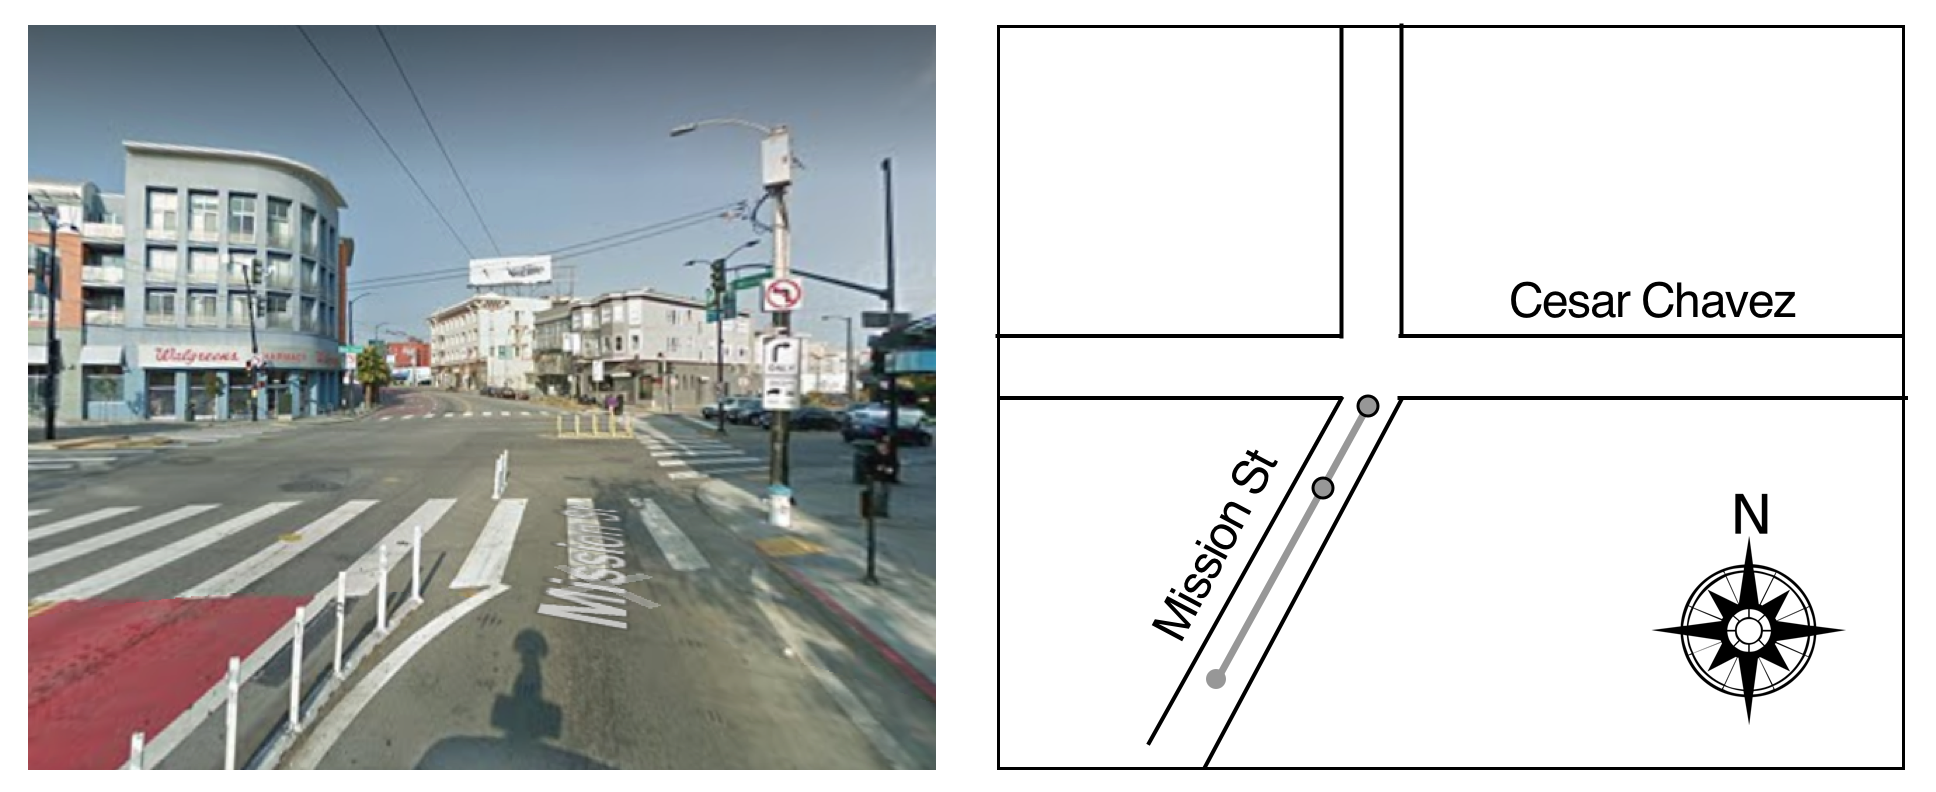
\includegraphics[width=\textwidth]{images/POLYLINE.png}
  \caption{Left: The Google Streetview image of the intersection of Mission and Cesar Chavez in San Francisco, part of the SF test set. Right: A map view of this intersection. The grey line is a polyline representative of the selected route leading into the intersection. To find the bearing value for the Torchbearer maneuver point we calculate the angle w.r.t. due north between the two points outlined in black.}
  \label{fig:polyline}
\end{figure}

Each maneuver point was processed through each of the four Torchbearer pipelines, resulting in a balanced result set of 1,600 pipeline executions.

\subsection{Marginal Cost}

Torchbearer pipelines incur monetary cost when they use MTurk to gather human input. In an effort to compare the drawbacks and benefits of each pipeline, it is important to have an understanding of the differences in expenditure.

Task workers record the cost incurred for the processing of each maneuver point as the pipeline executes in the Torchbearer database; anytime a HIT is submitted to MTurk the cost is increased by $nc$ where $n$ is the number of workers who will complete the HIT and $c$ is the amount to be paid to each worker. For this experiment we paid workers \$0.05 for a saliency selection HIT, \$0.05 for a landmark description HIT and \$0.03 for a landmark verification HIT. These amounts were selected based on observational analysis of Mechanical Turk pricing for similar object-detection-related tasks; we aimed to offer above average pay for each type of HIT to avoid low pay as a confounding variable in work quality. The marginal pipeline costs (the cost of processing an additional maneuver point) are shown in Figure \ref{fig:plot:cost}

\begin{figure}[htbp]
  \centering
  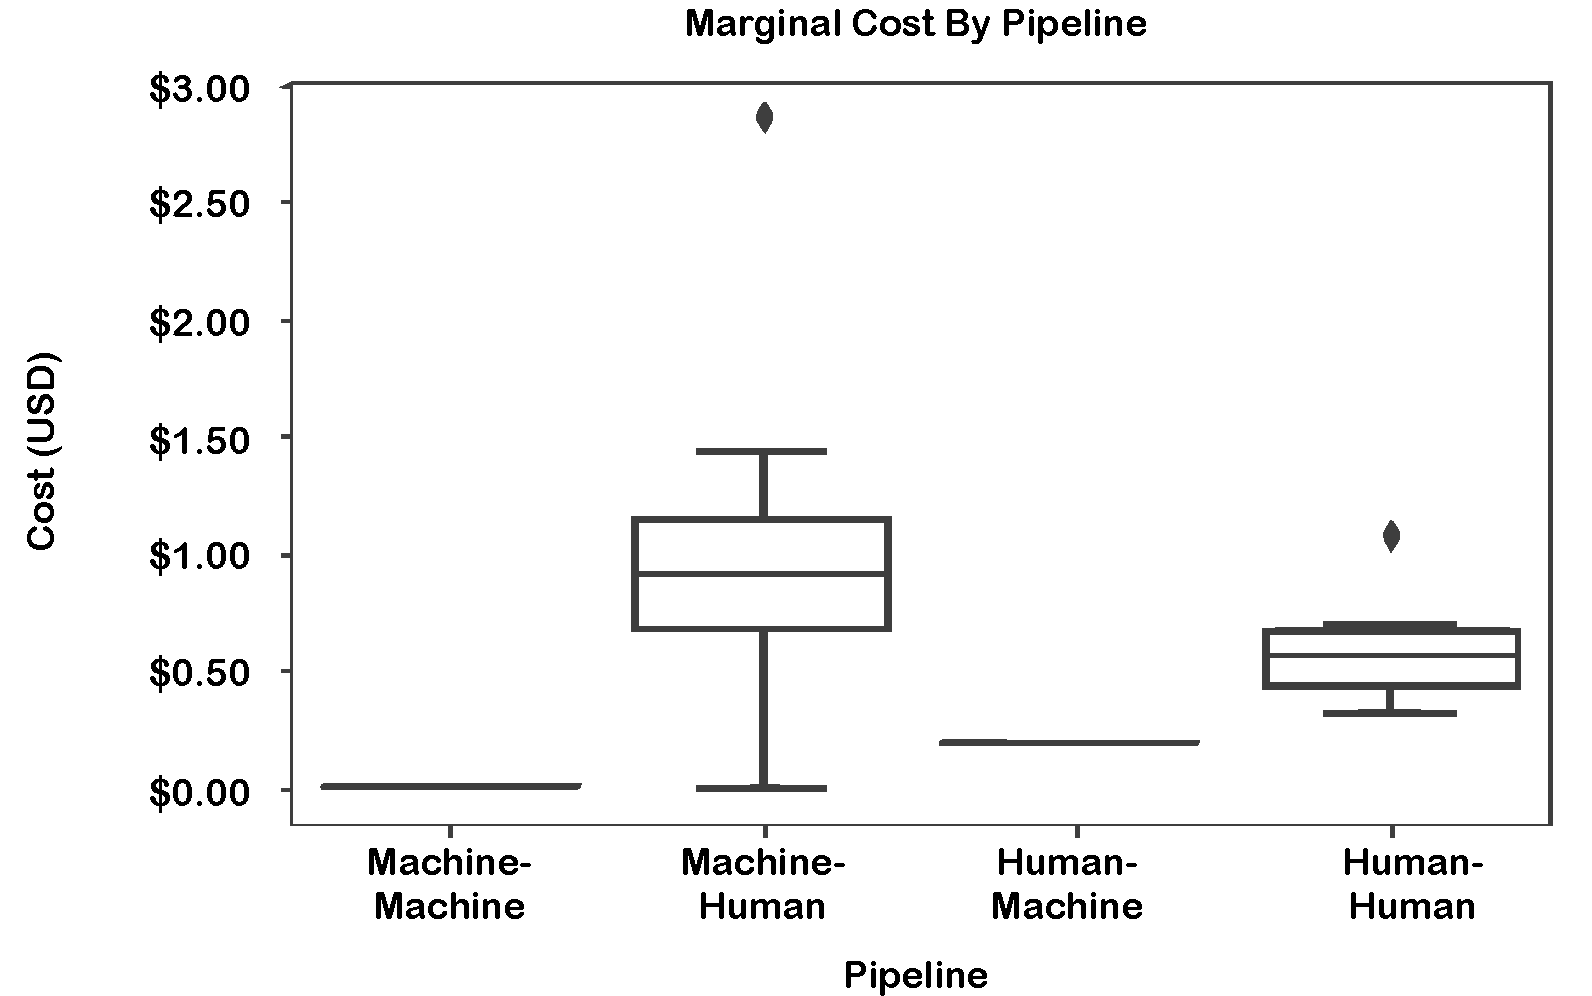
\includegraphics[width=\textwidth]{images/plot_cost.pdf}
  \caption{Marginal cost by pipeline}
  \label{fig:plot:cost}
\end{figure}

Based on the results of a one-way Analysis of Variance (ANOVA) test, we find that the mean marginal cost differs significantly by pipeline $F(3, 396)=154.59$, $p < 0.001$. A post-hoc analysis using Tukey Honest Significant Differences (HSD) reveals that, at $p < 0.05$, the marginal cost differs significantly between all pipelines except for the Machine-Machine and Human-Machine pipelines.

The marginal cost of the Machine-Machine pipeline is extremely low---it has a mean cost per maneuver point of \$0.00004. The Machine-Machine pipeline requires no human input, therefore the cost is entirely a result of computational resource usage: this pipeline takes on average of six seconds to execute form end-to-end, as will be seen in the following section, and the price of the AWS node upon which Torchbearer runs is \$0.02 per hour.  

The results for the Human-Machine pipeline are similarly deterministic---this pipeline requests a single saliency detection HIT with a fixed number of worker assignments (5 in our experiment). The Machine-Human pipeline exhibits not only the highest average cost, but also the highest variance. Both of these traits are due to the description verification component, which has the potential to repeat the entire description step, introducing non-determinism and increasing the cost of a execution significantly. 

This non-determinism due to verification is also a likely explanation of the variance observed in the Human-Machine pipeline. However, variance is less than the Machine-Human pipeline, which we attribute to humans' seeming ability to select more meaningful landmarks during the saliency step than the SalNet-based saliency approach. In other words, it is possible that the machine approach to saliency sometimes selects salient regions, which do not contain an object that can be easily described, and contention is created among and between the describing workers and verification workers. This leads to more ``loops" of the description step when workers don't agree, and therefore a higher execution cost.

The relatively high costs of the human-based pipeline may not render them impractical, however. Since the street-level imagery used by Torchbearer is not (currently) realtime, updated on a scale of years, a given maneuver point only needs to be processed by Torchbearer on a relatively rare frequency. Thus, if a particular pipeline proves to be expensive, but highly useful for drivers, it might be worth bearing that cost on an $n$-year cycle. Of course if realtime imagery is used, the Machine-Machine pipeline may be the only economically viable option. 

Torchbearer is able to amortize costs by storing landmark descriptions for every maneuver point it processes. Thus, only the first request for a given maneuver point/pipeline combination will require processing by the pipeline. Costs are amortized by the number of requests received between updates of the street-level imagery source.

\subsection{Execution Time}
Along with monetary cost, execution time is a cost to using a given pipeline. Using our San Francisco test set, we measure both end-to-end processing time and task-wise execution time.

\subsubsection{End-to-End Execution Time}
We record the start and end timestamps for each execution; the difference between these timestamps are shown in Figure \ref{fig:plot:executiontime}

\begin{figure}[htbp]
  \centering
  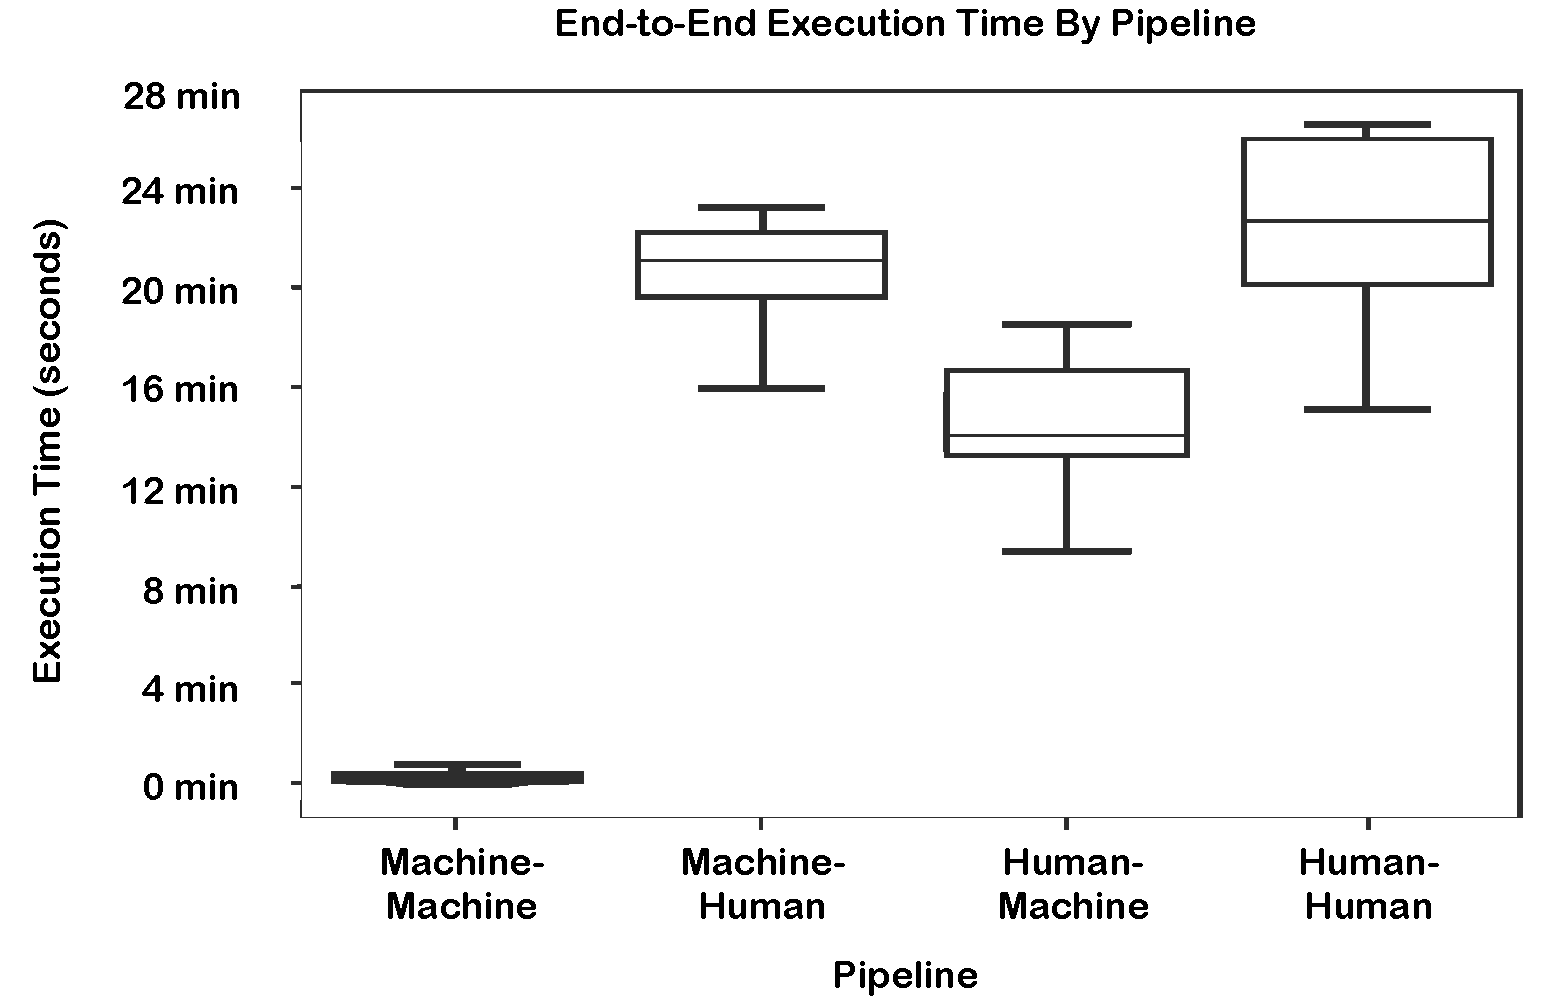
\includegraphics[width=\textwidth]{images/plot_executiontime.pdf}
  \caption{End-to-end execution time by pipeline}
  \label{fig:plot:executiontime}
\end{figure}

Based on the results of an ANOVA test, we find that the mean end-to-end differs significantly by pipeline $F(3, 396)=117.24$, $p < 0.001$. A post-hoc analysis using Tukey HSD reveals that, at $p < 0.05$, the end-to-end execution time differs significantly between all pipelines.

The Machine-Machine pipeline exhibits the lowest mean end-to-end execution time by an extreme margin, with very low variance. The pipelines which incorporate human input are, unsurprisingly, slower on the order of tens of minutes. These pipelines also exhibit significant variance, which is expected given the relative unpredictability of the human pipeline tasks. Likely for the same reasons we observe a higher marginal cost, we see a longer mean execution time for the Machine-Human pipeline than we do for the Human-Machine pipeline. The mean execution time for the Human-Human and Machine-Human pipelines are similar, again implying that the machine approach to saliency results in more looping, or contention, at the human description step. The Human-Human pipeline has the largest variance, due to the most reliance on human work, and also the highest time. 

Based on these results, it is likely that the only pipeline capable of executing at realtime speeds is the Machine-Machine pipeline. However, there a couple of nuances to consider: first, Mechanical Turk has the potential to become faster as Torchbearer continues to build up a pool of workers. (The more workers, the more likely an already-qualified worker will be at the ready when a Torchbearer HIT is submitted.) During the SF test set simulation, 47 workers completed saliency HITs, 37 completed description HITs and 64 completed verification HITs. Over time, as the reputation of Torchbearer as a fair, well-paying requester grew, and more workers completed the qualification process, more parallelization could occur at the human worker level.

Second, as noted in regards to pipeline cost, the benefits of a realtime pipeline will not be realized unless the street-level imagery source is also realtime, which Google Streetview is not. Indeed, most landmarks are permanent fixtures in the environment, and thus a Torchbearer pipeline only needs to process a given maneuver point whenever the street-level imagery is updated. This means that processing could be batched---an entire city's landmarks could be reevaluated at one time, and the per-maneuver point execution time of a pipeline is not relevant.

Third, for long trips it may be that a 20 to 30 minute processing time is acceptable for some landmarks. If a route consists of an hour of freeway driving, followed by several maneuver points in the destination city, the latter maneuver points can be processed while the user is on the freeway.

\subsection{Execution Time By Task}

For each pipeline, we evaluate the mean time required to complete each task. This gives insight into any bottlenecks that might exist in a pipeline, as well as the effectiveness of any task parallelization that was implemented. Each plot below represents an ``average timeline" of execution. The length of the horizontal bar shows the average execution time for the given task, laid out in the order of execution. The plot is arranged such that tasks which execute in parallel are shown with the same start time.

\subsubsection{Machine-Machine}
\begin{figure}[htbp]
  \centering
  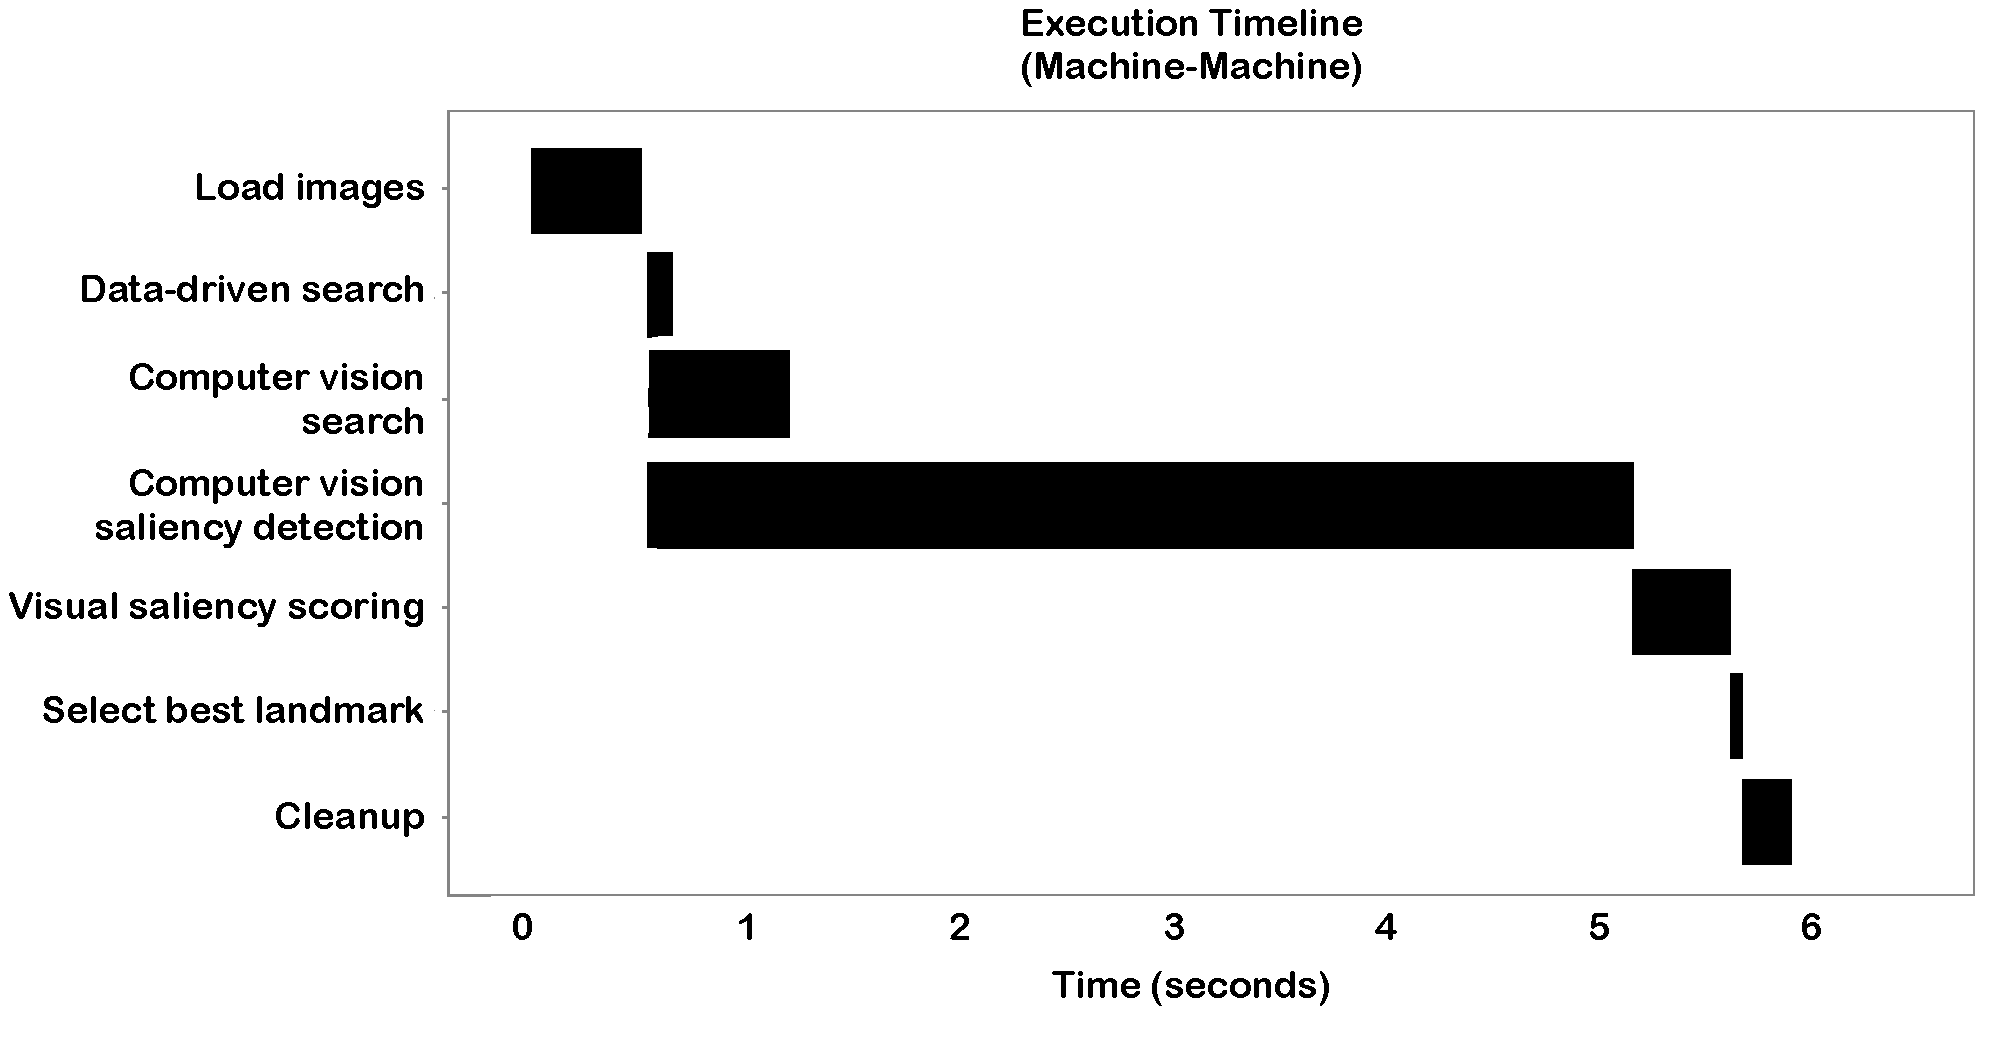
\includegraphics[width=\textwidth]{images/timeline_mm.pdf}
  \caption{Execution time by task (Machine-Machine pipeline)}
  \label{fig:plot:timeline:mm}
\end{figure}

Figure \ref{fig:plot:timeline:mm} shows that the lion's share of processing time in the Machine-Machine pipeline is devoted to the computer vision saliency (SalNet) task. This is unsurprising, as SalNet is a computationally-intensive algorithm, consisting of convolutional filters being applied across the street-level image many times. We also observe noticeable time reductions by parallelizing the saliency detection, computer vision search and data-driven search tasks.

\subsubsection{Machine-Human}
\begin{figure}[htbp]
  \centering
  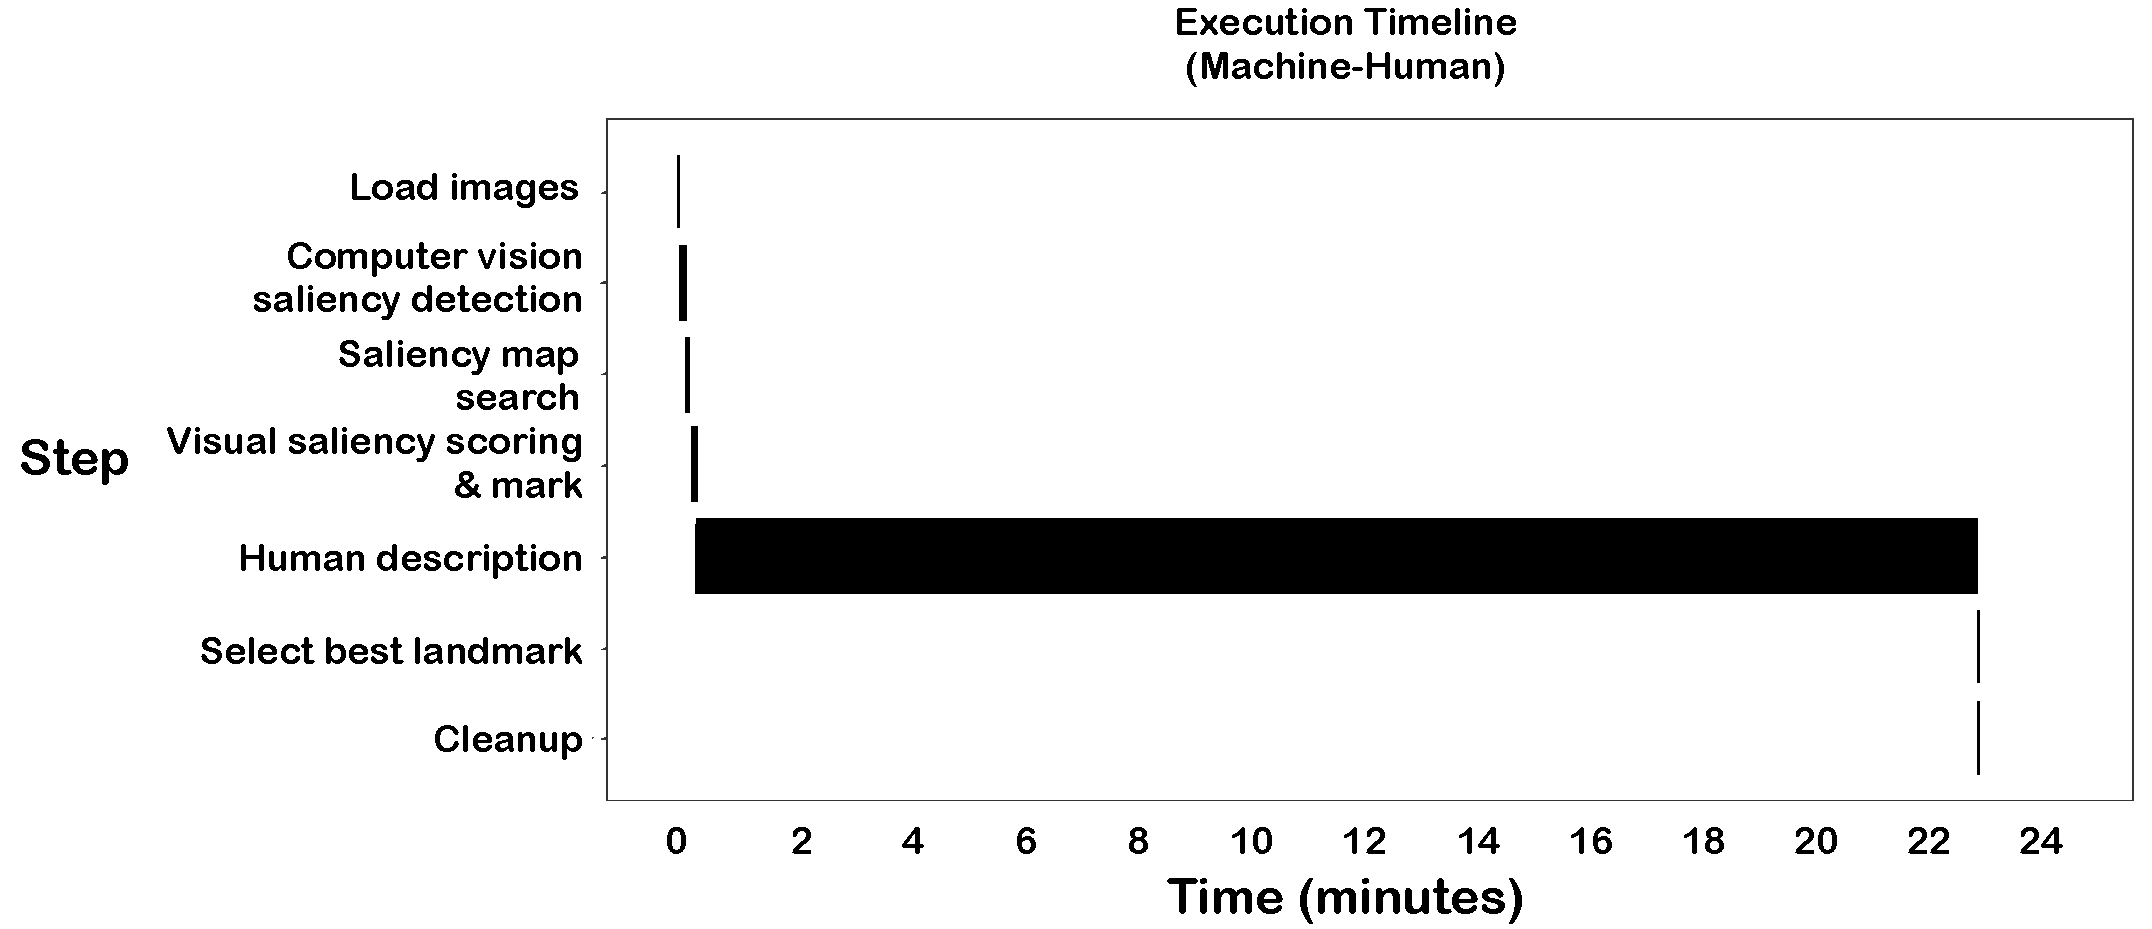
\includegraphics[width=\textwidth]{images/timeline_mh.pdf}
  \caption{Execution time by task (Machine-Human pipeline)}
  \label{fig:plot:timeline:mh}
\end{figure}

Figure \ref{fig:plot:timeline:mh} makes clear that the human landmark description task is the bottleneck in the Machine-Human pipeline, accounting for approximately 98\% of total execution time. Parallelization does not provide significant benefits in terms of end-to-end execution time.

\subsubsection{Human-Machine}
\begin{figure}[htbp]
  \centering
  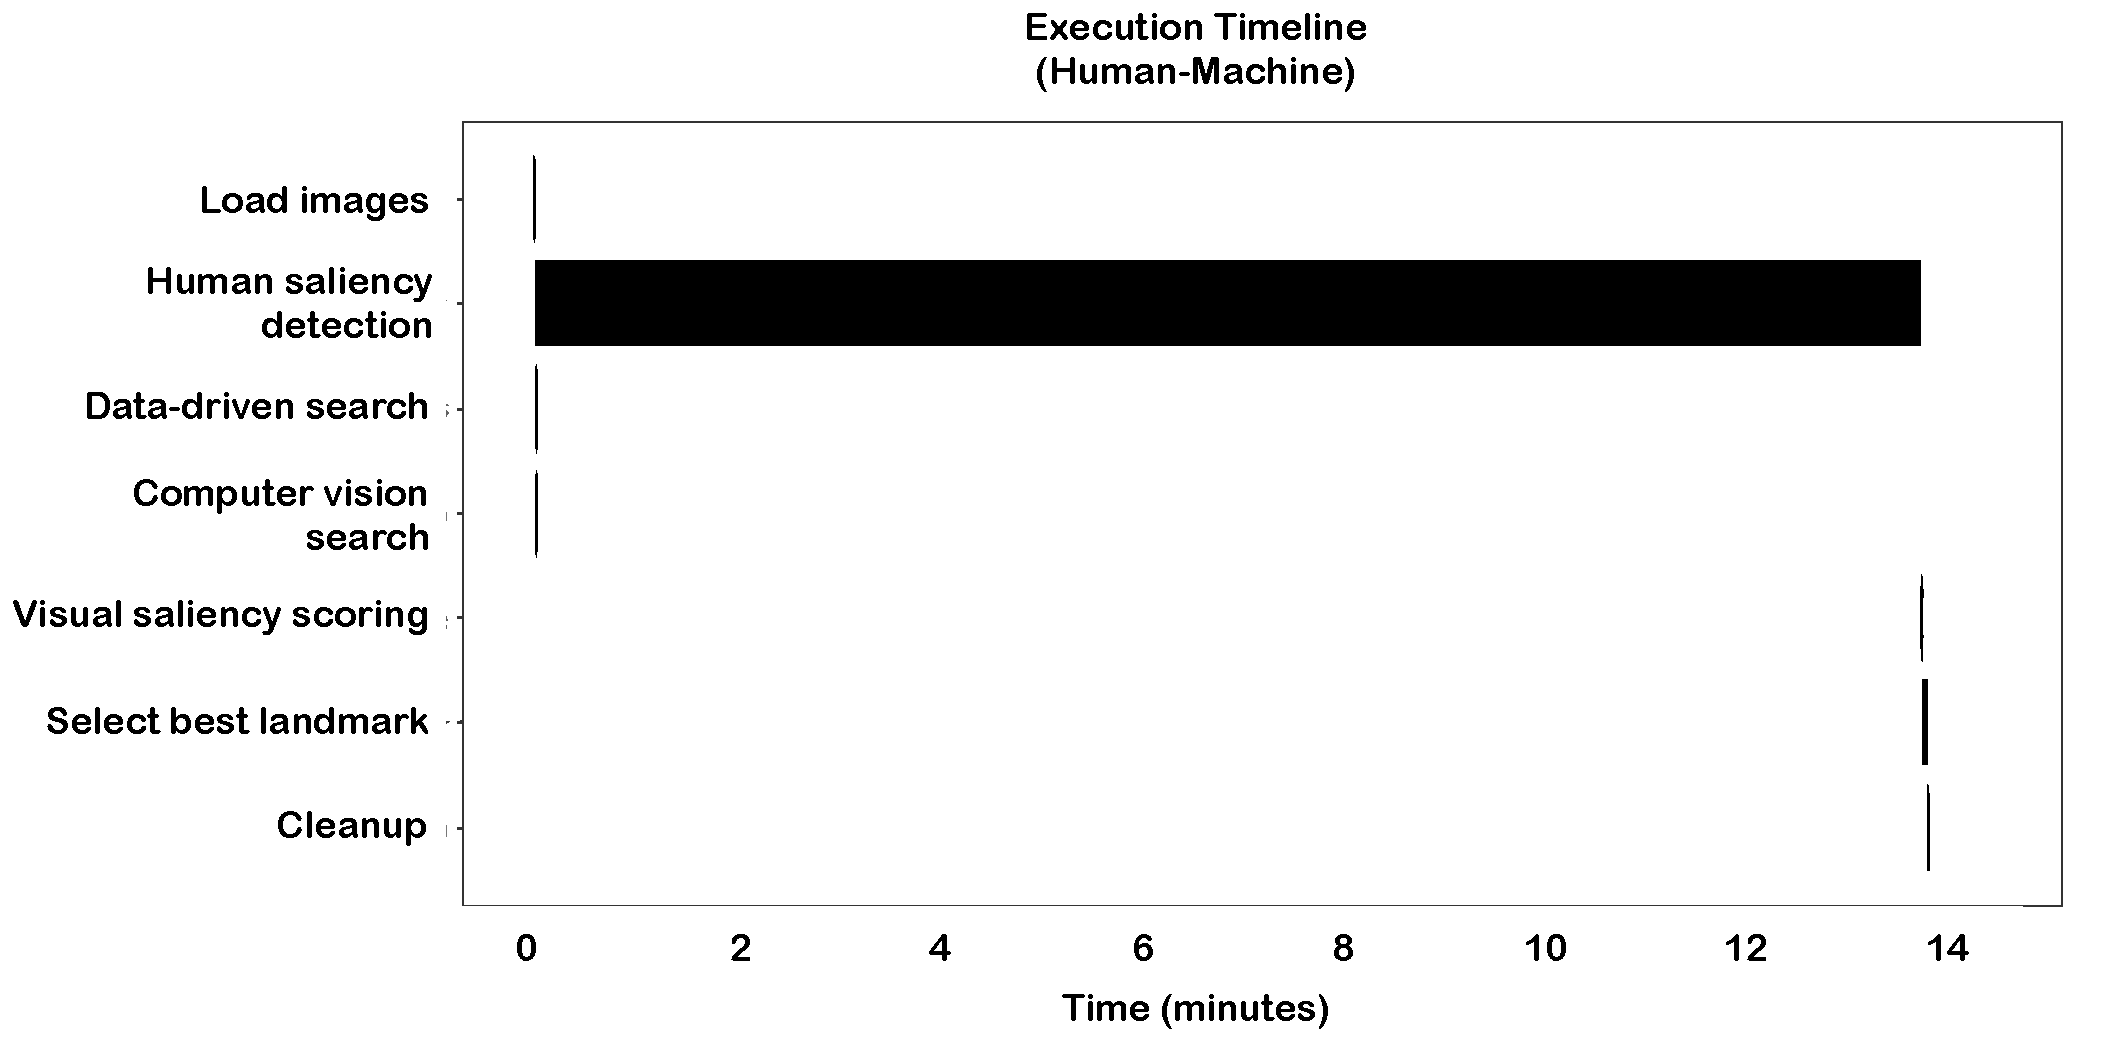
\includegraphics[width=\textwidth]{images/timeline_hm.pdf}
  \caption{Execution time by task (Human-Machine pipeline)}
  \label{fig:plot:timeline:hm}
\end{figure}

Figure \ref{fig:plot:timeline:hm} shows that the Human-Machine pipeline suffers from a single bottleneck in the form of the human saliency task, which is to be expected as all other tasks required no human input. While some tasks are parallelized, the effect of this on the overall execution time is negligible.

\subsubsection{Human-Human}
\begin{figure}[htbp]
  \centering
  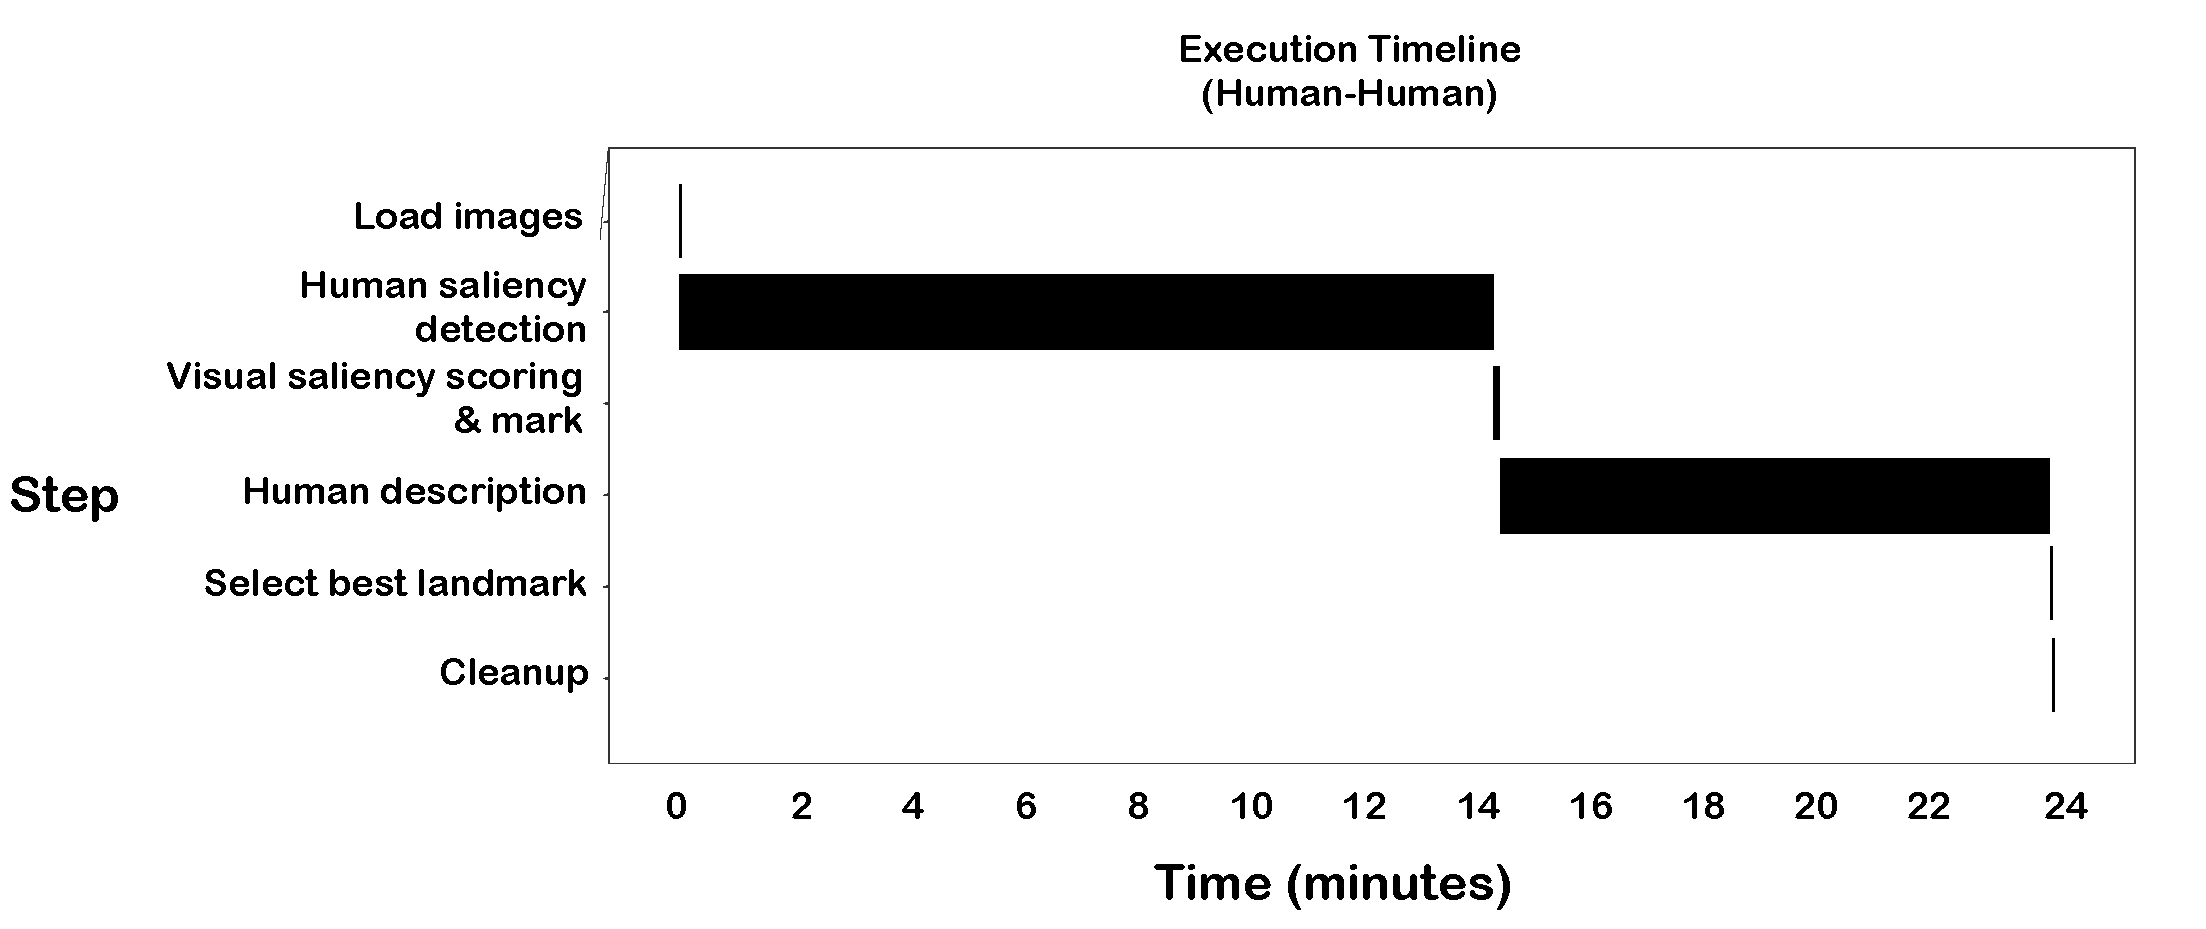
\includegraphics[width=\textwidth]{images/timeline_hh.pdf}
  \caption{Execution time by task (Human-Human pipeline)}
  \label{fig:plot:timeline:hh}
\end{figure}

In Figure \ref{fig:plot:timeline:hh}, it is clear that the two human-based tasks comprise the majority of execution time. The duration of the saliency task is somewhat longer than the description task, which we attribute to the number of workers required, as well as the difficulty of each task: the saliency task requires a sample of five workers, each of who had to make a somewhat involved decision about where to draw a box. The description task, on the other hand, requires a single worker to write a description, and three more to simply approve of what she wrote. While the description task does have the potential to ``loop" if the description is rejected, in the single-iteration case this task requires less workers, performing an easier task, than the saliency task does.

\subsection{Selected Landmark Overlap}

Every pipeline eventually selects a landmark, inclusive of a bounding box within the street-level image outlining its location. By comparing the intersection-over-union (IoU) between two landmark bounding boxes we can see to what degree the bounding boxes are selecting the same area. IoU is the ratio of area overlapped by both bounding boxes to the area encompassed by both bounding boxes; thus an IoU of 1 signifies complete agreement, or overlap, and an IoU of 0 indicates no overlap. IoU is expressed as
\begin{equation}
    IoU = \frac{area(intersection(b_1,b_2))}{area(union(b_1,b_2))}
\end{equation}
where $b_1$ and $b_2$ are the bounding boxes of two selected landmarks. Figure \ref{fig:iou} shows the intersection and the union of two hypothetical bounding boxes.

\begin{figure}[htbp]
  \centering
  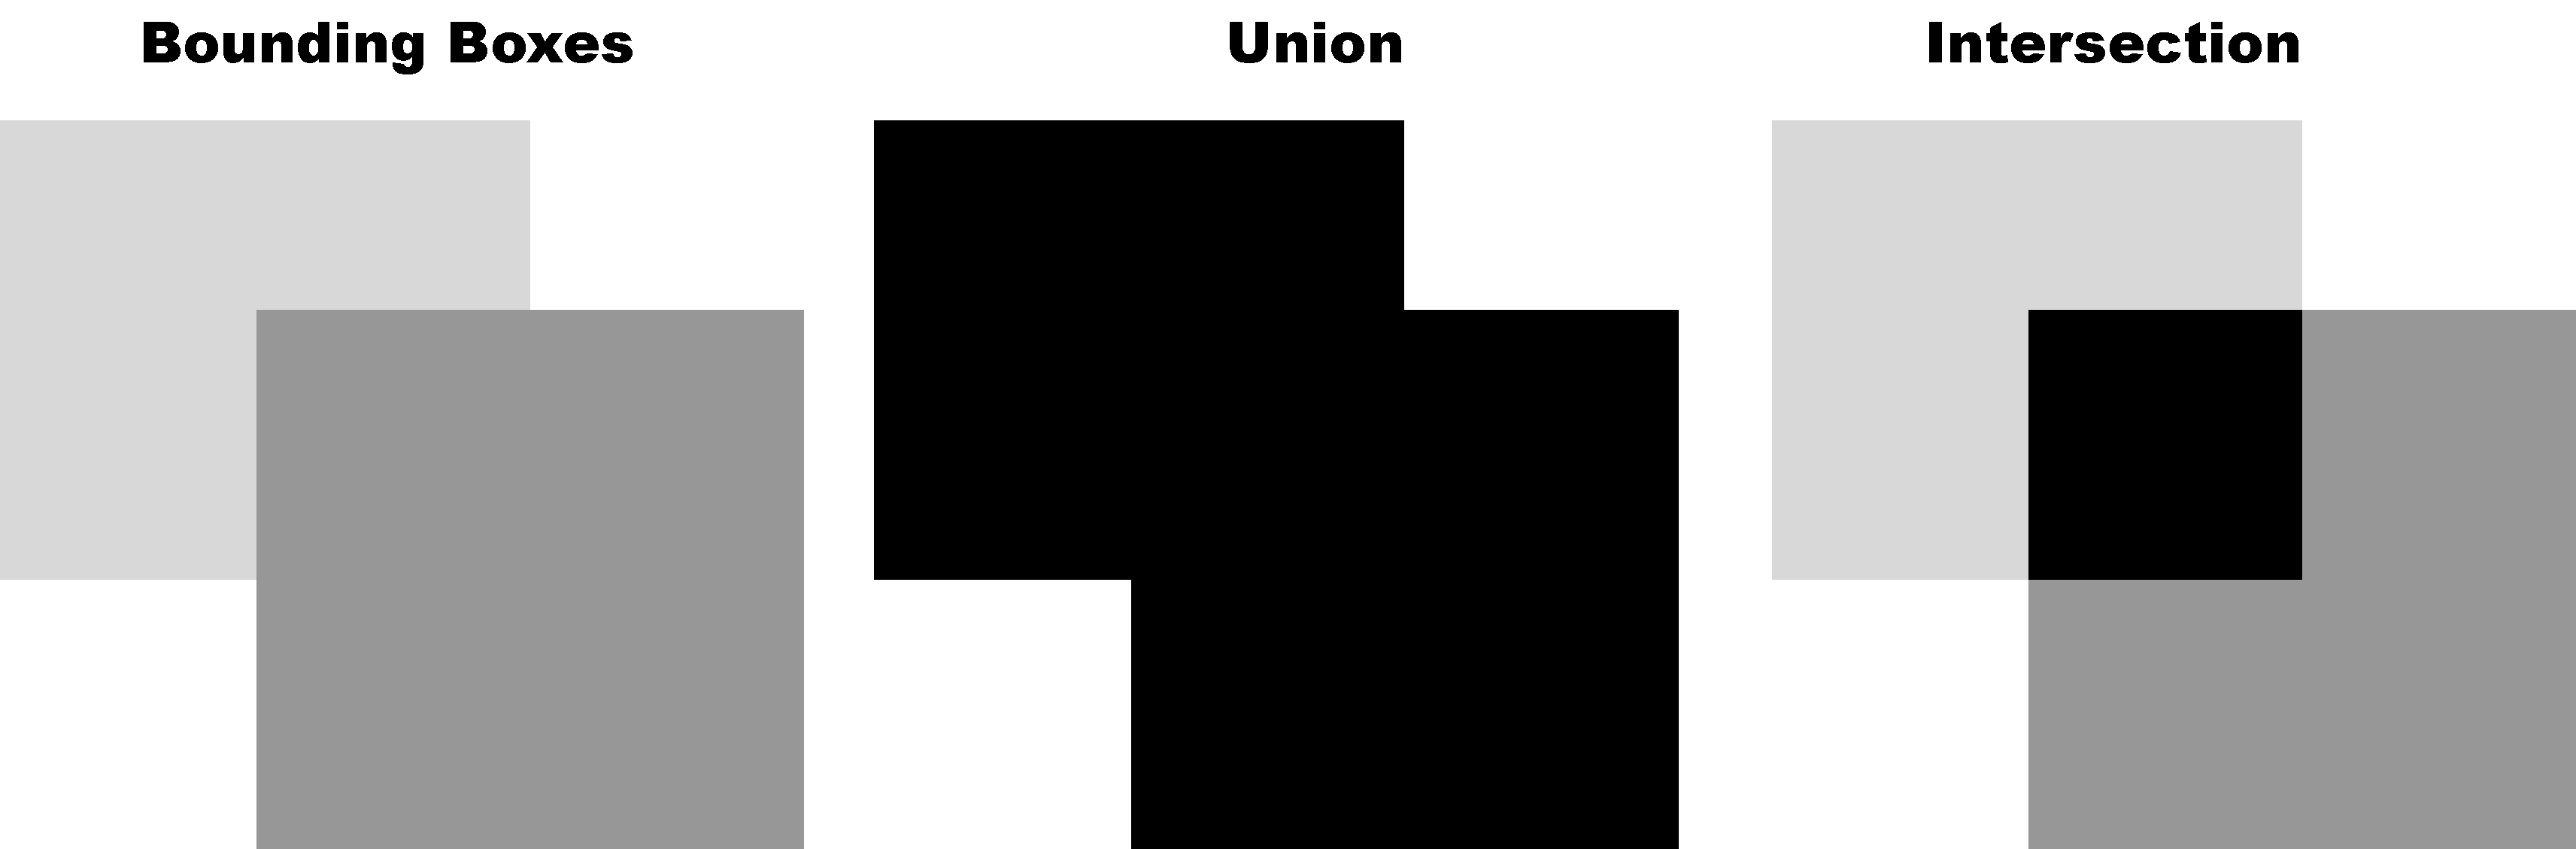
\includegraphics[width=\textwidth]{images/iou.pdf}
  \caption{The intersection (right) and union (center) of a pair of hypothetical bounding boxes (left). The black area selection represents the area of the given metric.}
  \label{fig:iou}
\end{figure}

\begin{table}[htbp]
  \centering
  \caption{Mean Intersection Over Union of Selected Landmark}
  \label{tab:iou}
  {\tabulinesep=2mm
    \begin{singlespace}
    \begin{tabu} to \textwidth{|X[c]||X[c]|X[c]|X[c]|}
    \hline
                & Machine-Human & Human-Machine & Human-Human \\
                \hline\hline
Machine-Machine   & 0.35        & 0.65          & 0.08          \\
\hline
Machine-Human &             & 0.07          & 0.09          \\
\hline
Human-Machine   &             &               & 0.05 
\\
    \hline
    \end{tabu}
    \end{singlespace}
    }
\end{table}

For each maneuver point in the SF test set, we compute the IoU between the selected landmark returned from each pipeline. Table \ref{tab:iou} shows the mean IoU between each pair of pipelines across all maneuver points. This is essentially a measure of how likely two pipelines were to select the same landmark, or, looked at another way, the agreement between two pipelines in terms of landmark saliency.

The mean IoU between landmarks selected by the Machine-Machine and Human-Machine pipelines is the highest, at 0.65; which we largely attribute to the pipelines' identical method of selecting candidate landmarks---object detection via Faster-RCNN and FourSquare venue search. Interestingly, the methods used for determining saliency, and selecting the best landmark, vary: while Human-Machine considers only saliency as determined by human workers, Machine-Machine considers a componentized saliency score with input from SalNet and semantic saliency based on checkins and ubiquity. This implies that, at least to some degree, humans agree with our componentized saliency method in regards to what makes the best landmark.

A high IoU also exists between the Machine-Machine and Machine-Human pipelines, suggesting agreement between the salient regions generated by SalNet, which define the candidate landmark set for the Machine-Human pipeline, and the object-detection algorithm and/or the FourSquare venue search, which together build the candidate set for the Machine-Machine pipeline.

For other pipeline combinations, the mean IoU is low enough that is unlikely to be more significant than random chance. However, even though different pipelines identify different landmarks, they could still provide utility to drivers. This is examined in the following section.


\iffalse
\subsection{Description Similarity}

Pipelines use two separate methods for describing candidate landmarks: human-based, in which human workers provide free-form text in response to an image of the landmark, and machine-based, where the description is generated by an object-detection algorithm or the venue description in a database. To analyze the similarity between descriptions generated for identical landmarks across pipelines, we leverage the same word embedding approach used for computing landmark uniqueness (see \ref{sec:unique}. 

Considering only those landmarks which had an IoU of greater than 0.5, we compute the vector space embedding for each generated description, and then find the cosine similarity between those two embeddings. Table \ref{tab:descriptionsimilarity} reports the mean cosine similarity between landmark description for each pair of pipelines.

\begin{table}[htbp]
  \centering
  \caption{Mean Cosine Similarity Between Selected Landmarks (normalized between [0,1])}
  \label{tab:descriptionsimilarity}
  {\tabulinesep=2mm
    \begin{singlespace}
    \begin{tabu} to \textwidth{|X[c]||X[c]|X[c]|X[c]|}
    \hline
                & Machine-Human & Human-Machine & Human-Human \\
                \hline\hline
Machine-Machine & 0.21 & 0.68 & 0.19 \\
    \hline
Machine-Human   &      & 0.17 & 0.56 \\
    \hline
Human-Machine   &      &      & 0.18
\\
    \hline
    \end{tabu}
    \end{singlespace}
    }
\end{table}

\fi

\section{Field Experiments}

To evaluate the efficacy of each of our approaches for reducing driver cognitive load and improving driving performance, we conduct a Institutional Review Board approved instrumented-vehicle driving study (real driver, real vehicles, real roads) in which subjects navigate along a route unknown to them using the Torchbearer system. (The Human Subjects Consent Form for these experiments can be found in Appendix \ref{append:consent}.) It must be noted up front that, due to constraints on time and resources, a full-scale human factors study is out of the scope of this work. While the experimental design we discuss could be applied to a larger sample and potentially yield significant results, here we use a sample size of five human subjects. Along with contributing a experimental design for future work, this small-scale study provides exploratory evidence as to the effectiveness of the Torchbearer system.

\subsection{Experimental Design}

We evaluate each of Torchbearer's four pipelines against a control pipeline which delivers instructions containing no landmarks. The control pipeline is comparable to a mainstream navigation application, such as Google Maps, which provides only street names and distances in its instructions.

Using a within-subjects design, five subjects drove an identical route through downtown Bozeman, Montana, using only the Torchbearer app for navigation (shown in Figure \ref{fig:route}). The route was selected due to its grid (city block) layout, offering many locations for turns and a wide variety of landmarks (residential, business, and street infrastructure.) It allowed for incorporating a large number of maneuvers into the allocated 60-minute experiment time frame. This route was divided into five legs, with a different pipeline being used for navigation of each leg. After the completion of each leg, the subject was given asked to complete the NASA-TLX survey, to measure perceived task load for that leg and pipeline. A sample of landmarks used for each pipeline and route leg can be seen in Appendix \ref{appendix:route}.

\begin{figure}[htbp]
  \centering
  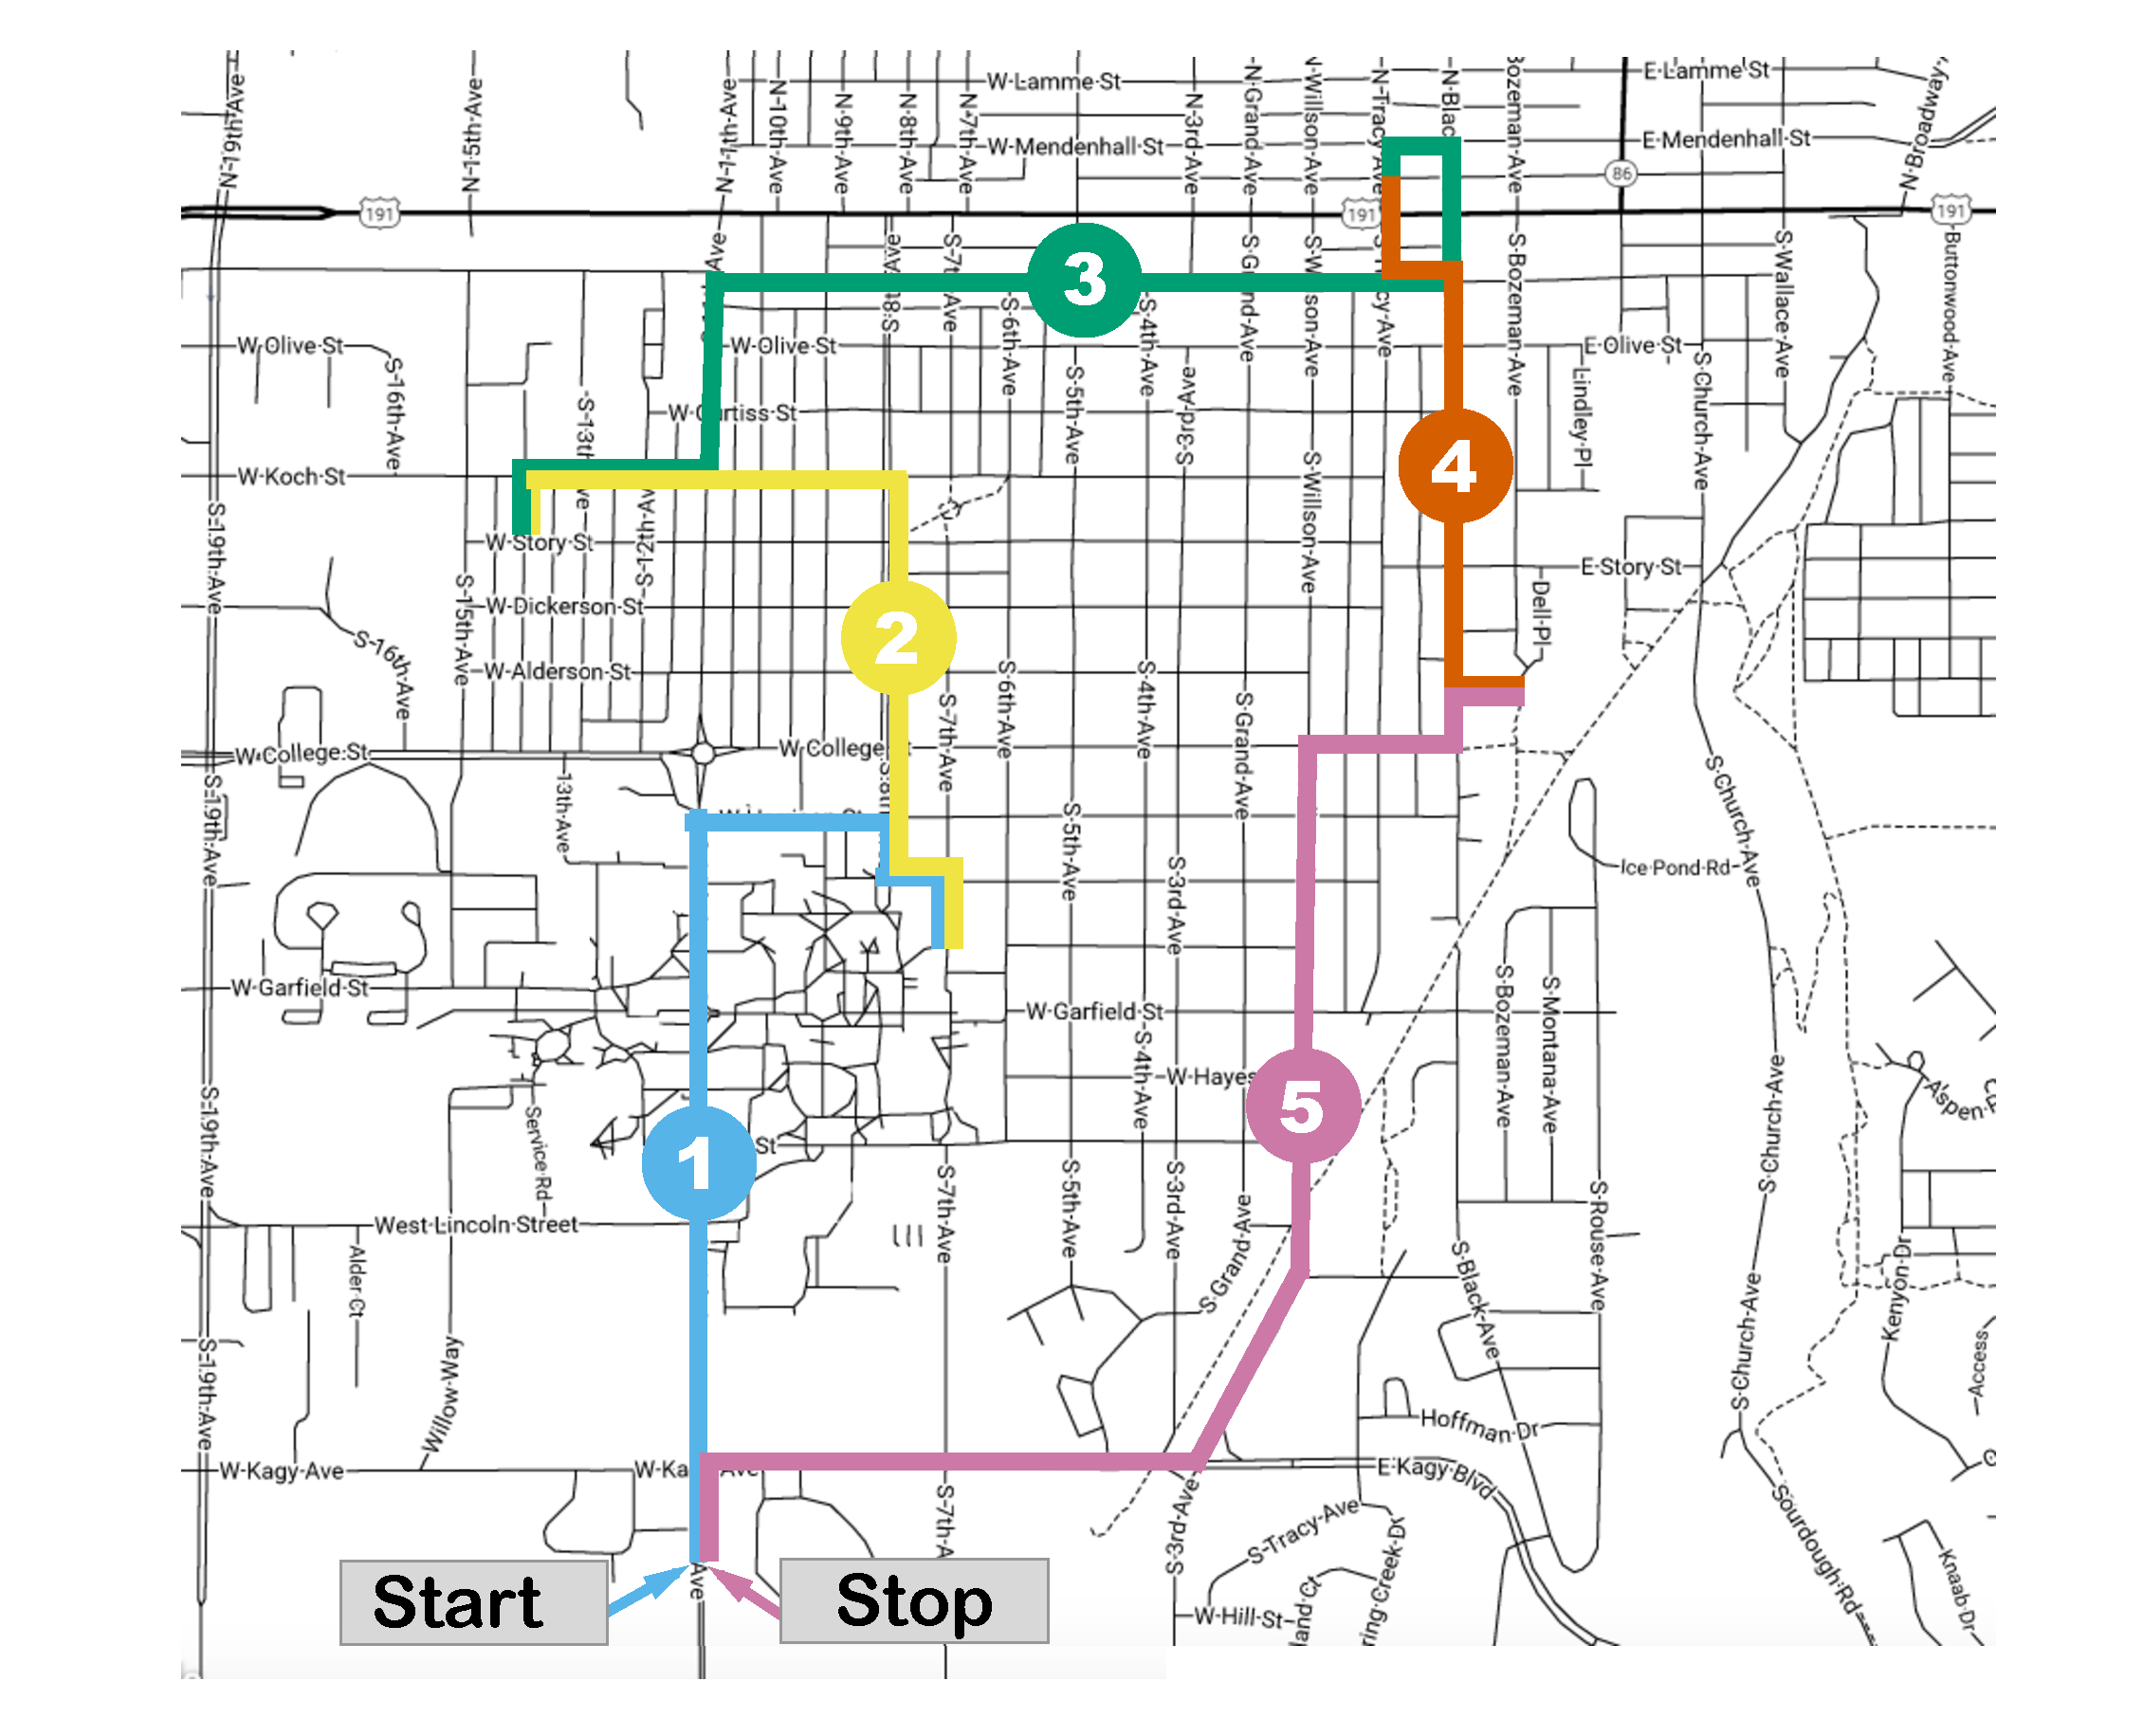
\includegraphics[width=0.8\textwidth]{images/route.pdf}
  \caption{The route driven by subjects through Bozeman, Montana. Each color represents a different leg. Each leg is navigated using a different pipeline.}
  \label{fig:route}
\end{figure}

The subject was given no information about the route prior to the start of driving; the only information they were given throughout the drive was spoken by the Torchbearer app. Subjects were all white; two were male and three were female. All indicated they had at least some familiarity with the area of Bozeman in which the test route was located. Subjects were not compensated.

Our experiment has two sources of nuisance variability, or blocking factors: the route leg and the subject (driver). Each leg of the route is likely to have differences in road type, normal traffic levels and availability of good landmarks. Subjects vary in their driving abilities, driving style (tendency to brake hard, turn quickly, etc.), preexisting knowledge of the area in which the experiment is conducted, as well as global factors such as the time of day, weather, or traffic levels at the time the subject completed the trials. All of these characteristics can have an undesired effect on the variable of interest. 

To control for these two blocking factors, we use a Latin squares design, which allows for controlling two sources of variation---subject and route leg---and isolates the treatment effect (pipeline). This is accomplished by requiring that each pipeline be analyzed on all route legs an equal number of times, and also that each subject be treated with each pipeline an equal number of times. A Latin square can be thought of as an $n$ by $n$ matrix, where rows represent a subject and columns represent a route leg, and $n$ is equal to the number of pipelines, subjects and route legs (five).

The standard Latin squares design does not control for the effects of treatment order---the carryover effect of subjects always being treated with pipeline $x$ after pipeline $y$---so we use a counterbalanced Latin square, which carries the additional stipulation that each pipeline must be preceded by and followed by every other pipeline an equal number of times. That is, if $p_y$ is \textit{preceded} by $p_x$ for one subject, $p_y$ must be \textit{followed} by $p_x$ for exactly one subject.

Because we have an odd number of treatments (four Torchbearer pipelines and one control pipeline) it is not possible to achieve the counterbalancing stipulation within an $n$ by $n$ Latin square. Instead, two $n$ x $n$ Latin squares, with the second being a vertical reflection of the first, are required. This results in a $2n$ by $n$ matrix, still with $n$ route legs and $n$ pipelines, but now requiring $2n = 10$ subjects. Because the scope of our study is limited to 5 subjects, we counterbalance the $5$ by $5$ to the greatest extent possible, but still have some immediate orderings which do not have the reverse represented in the square. This is a weakness of our study, and an argument in favor of future work with a larger pool of subjects, but we argue it will not threaten validity to a greater extent than the small sample size. Our Latin square design is displayed in Table \ref{tab:latinsquares}.

Using the Latin square design, we arrive at the following statistical model:
\begin{equation}\label{eq:model}
    Y_{ijk} = \overline{Y} + P_i + R_j + S_k + e_{ijk}
\end{equation}
where $\overline{Y}$ is the grand mean, $P_i$ is the pipeline (treatment) effect for a particular pipeline $i$, $R_j$ is the route leg effect for a particular route leg $j$, $S_k$ is the subject effect for a particular subject $k$, $e$ is the error term and $Y_{ijk}$ is an observation for a particular subject, route leg and pipeline.

\begin{table}[htbp]
  \centering
  \caption{Counterbalanced Latin Squares Design}
  \label{tab:latinsquares}
  {\tabulinesep=2mm
    \begin{singlespace}
    \begin{tabu} to \textwidth{|X[c]||X[c]|X[c]|X[c]|X[c]|X[c]|}
        \hline
        & Leg 1 & Leg 2 & Leg 3 & Leg 4 & Leg 5 \\
        \hline\hline
        Subject 1 & No landmarks    & Human-Human     & Machine-Machine & Human-Machine   & Machine-Human   \\
                \hline
        Subject 2 & Human-Human     & Human-Machine   & No landmarks    & Machine-Human   & Machine-Machine \\
                \hline
        Subject 3 & Human-Machine   & Machine-Human   & Human-Human     & Machine-Machine & No landmarks    \\
                \hline
        Subject 4 & Machine-Human   & Machine-Machine & Human-Machine   & No landmarks    & Human-Human     \\
                \hline
        Subject 5 & Machine-Machine & No landmarks    & Machine-Human   & Human-Human     & Human-Machine   \\
    \hline
    \end{tabu}
    \end{singlespace}
    }
\end{table}

\subsubsection{Peripheral Detection Task}

To measure the effect of pipelines' landmark descriptions on cognitive load, we use a peripheral detection task (PDT). This secondary task consists of subjects wearing a headset, which positions an LED light approximately 15 degrees to the left of the center of vision and 2 degrees above the horizon. This light blinks at a uniform random interval between 3 and 5 seconds, for a duration of between 200 and 1000 milliseconds \cite{martens2000measuring}. A button is attached to the subject's finger, which can be pressed against the steering wheel. The subject is asked to depress the button as quickly as possible whenever they see the light blink. The average delay between light blink and button depression is recorded, along with a miss rate---if the subject fails to press the button within 2 seconds of a light blink, it counts as a miss. Intuitively, the more cognitive effort the subject must expend on the primary task of navigation and vehicle operation, the less effort they can put towards the PDT. Thus, a more cognitively-intensive primary task will result in a higher miss rate and longer button press delay.

The PDT must be evaluated on two levels---first the miss rate, the probability of a subject never pressing the button within 2 seconds of the LED blinking, and second the mean response time for non-missed blinks.

Using a Kruskal-Wallis evaluation based on the linear model in Equation \ref{eq:model}, where $Y$ is the PDT response time, we found no evidence supporting a difference in mean PDT response time between pipelines ($F(4, 12) = 1.38$, $p=0.29$). We use Kruskal-Wallis in place of ANOVA because the normality assumption is violated (by visual analysis of the Q-Q plot). Figure \ref{fig:plot:responsetime} shows that differences in the mean are small relative to the large interquartile range.

\begin{figure}[htbp]
  \centering
  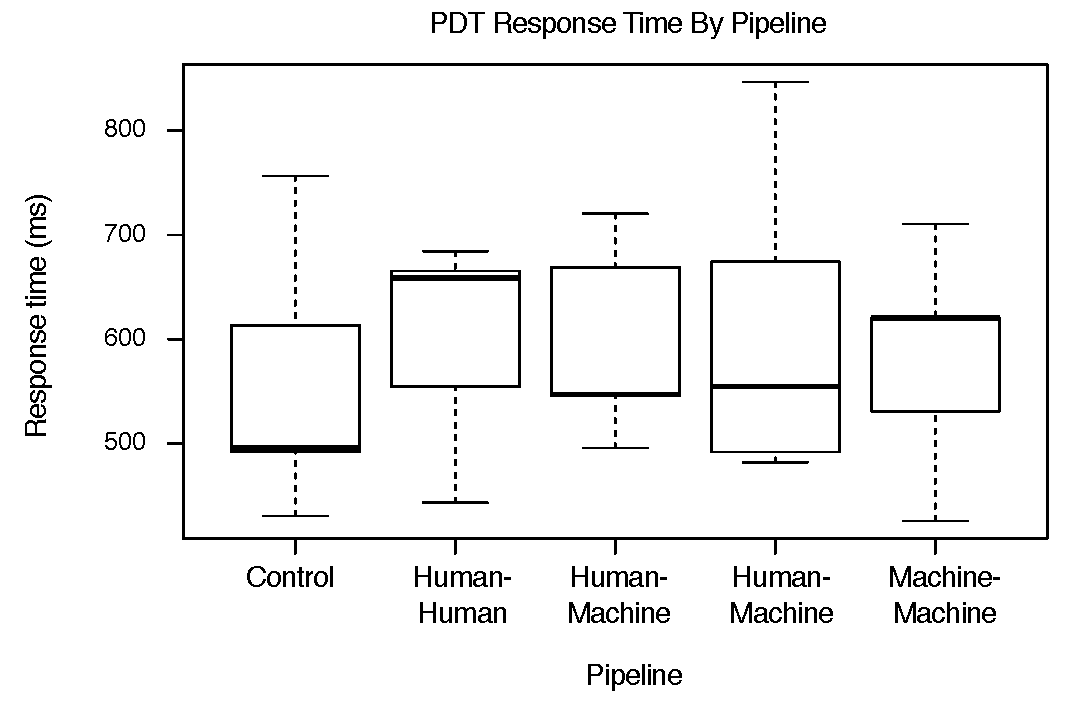
\includegraphics[width=0.6\textwidth]{images/plot_responsetime.pdf}
  \caption{PDT response time by pipeline}
  \label{fig:plot:responsetime}
\end{figure}

We also found no evidence of pipeline affecting PDT miss rate ($F(4, 12) = 0.46$, $p=0.76$), using the same analysis as for response time. (The normality assumption was violated for this data as well.) Figure \ref{fig:plot:missrate}  shows the distribution of miss rate by pipeline.

\begin{figure}[htbp]
  \centering
  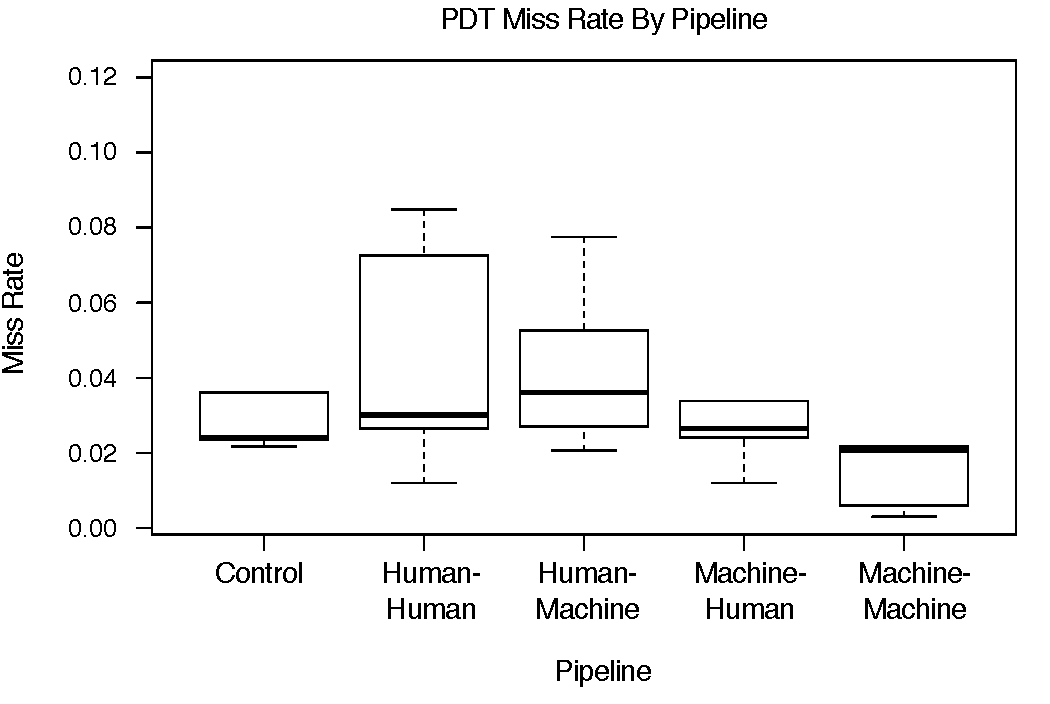
\includegraphics[width=0.6\textwidth]{images/plot_misses.pdf}
  \caption{PDT miss rate by pipeline}
  \label{fig:plot:missrate}
\end{figure}

\subsubsection{Gravitational Force Events}
We also monitor for erratic, harsh, potentially dangerous driving patterns, by counting instances of high lateral ($X$) and longitudinal~($Y$) gravitational forces (G-forces). These G-force spikes, which we call \textit{excessive force events} can signify harsh breaking, rapid acceleration or swerving. Specifically, we count the number of times during a route leg that the vehicle experienced a G-force of greater magnitude than the thresholds set forth in Table \ref{tab:acc}. G-forces are measured in the $X$ and $Y$ directions using a Freematics ONE vehicle data logger, which includes 3-axis acceleration data and is anchored to the vehicle frame via the vehicle's OBD-II port.

\begin{table}[htbp]
  \centering
  \caption{Gravitational Force Event Thresholds (Naturalistic Teenage Driving Study \cite{doi:10.1093/aje/kwr440})}
  \label{tab:acc}
  {\tabulinesep=2mm
    \begin{singlespace}
    \begin{tabu} to \textwidth{|X[c]|X[c]|X[c]|}
        \hline
        Event Type & Axis & Threshold (G) \\
        \hline\hline
        Harsh acceleration & $Y$ & $>0.35$ \\
        \hline
        Hard braking & $Y$ & $<-0.45$ \\
        \hline
        Right swerve & $X$ & $>0.05$ \\
        \hline
        Left swerve & $X$ & $<-0.05$ \\
    \hline
    \end{tabu}
    \end{singlespace}
    }
\end{table}

Using the same analysis as for the PDT metrics, we found no evidence that pipeline affects the number of excessive force events occurring during a drive ($F(4, 12) = 1.44$, $p=0.28$). See Figure \ref{fig:plot:acc}.

\begin{figure}[htbp]
  \centering
  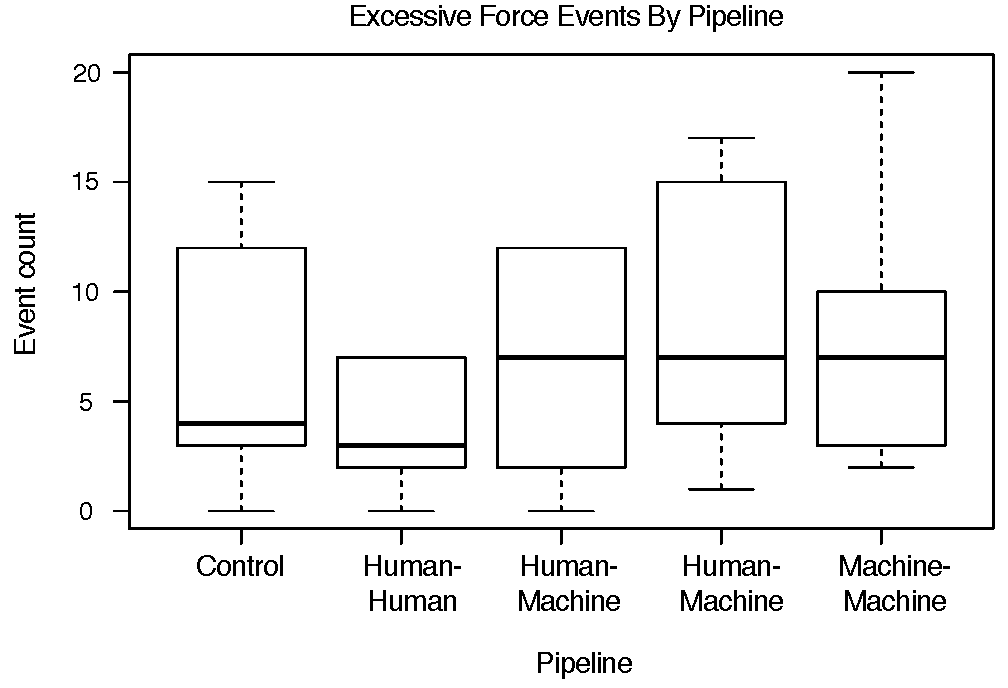
\includegraphics[width=0.6\textwidth]{images/plot_acc.pdf}
  \caption{Gravitational force events by pipeline}
  \label{fig:plot:acc}
\end{figure}

\subsubsection{Surveys}
Lastly, we survey subjects using the NASA-TLX survey \cite{hart1988development} and our own Likert-scale survey to analyze perceived task difficulty, as well as perceived landmark goodness, navigation confidence, and navigation difficulty between pipelines. Both surveys were administered for each pipeline, immediately following the completion of each leg.

The NASA-TLX survey consists of six sub-scales, which when combined aim to measure the total workload induced by the task---in this case navigating a route leg from start to finish using a particular pipeline for navigation. The scales are ordinal, with 20 levels ranging from \textit{very low} to \texit{very high}. (See Appendix \ref{appendix:tlx} for a full copy of the NASA-TLX survey.) The sub-scales are \textit{mental demand}, which measures the mental and perceptual acuity required to complete the task; \textit{physical demand}, which gauges how strenuous the task was; \textit{temporal demand}, which measures perceived time pressure or rush to complete the task; \textit{overall performance}, which indicates the subject's opinion of how successful she was at completing the task; \textit{effort}, a combined measure of mental and physical exertion; and \textit{frustration level}, how annoyed and irritated the subject felt during the task \cite{hart1988development}. \textbf{It is very important to note that the Performance sub-scale considers level 0 to equate to total success and level 20 to total failure, the opposite of what one might expect.}

We evaluate each sub-scale independently, so that individual effects can be parsed out. Figure \ref{fig:plot:tlx} shows the score distributions by pipeline, across each sub-scale. Because the scales are ordinal, we use the non-parametric Kruskal-Wallis analysis of variance to test for differences between pipelines. Table \ref{tab:tlx} lists the results across each sub-scale.

\begin{figure}[htbp]
  \centering
  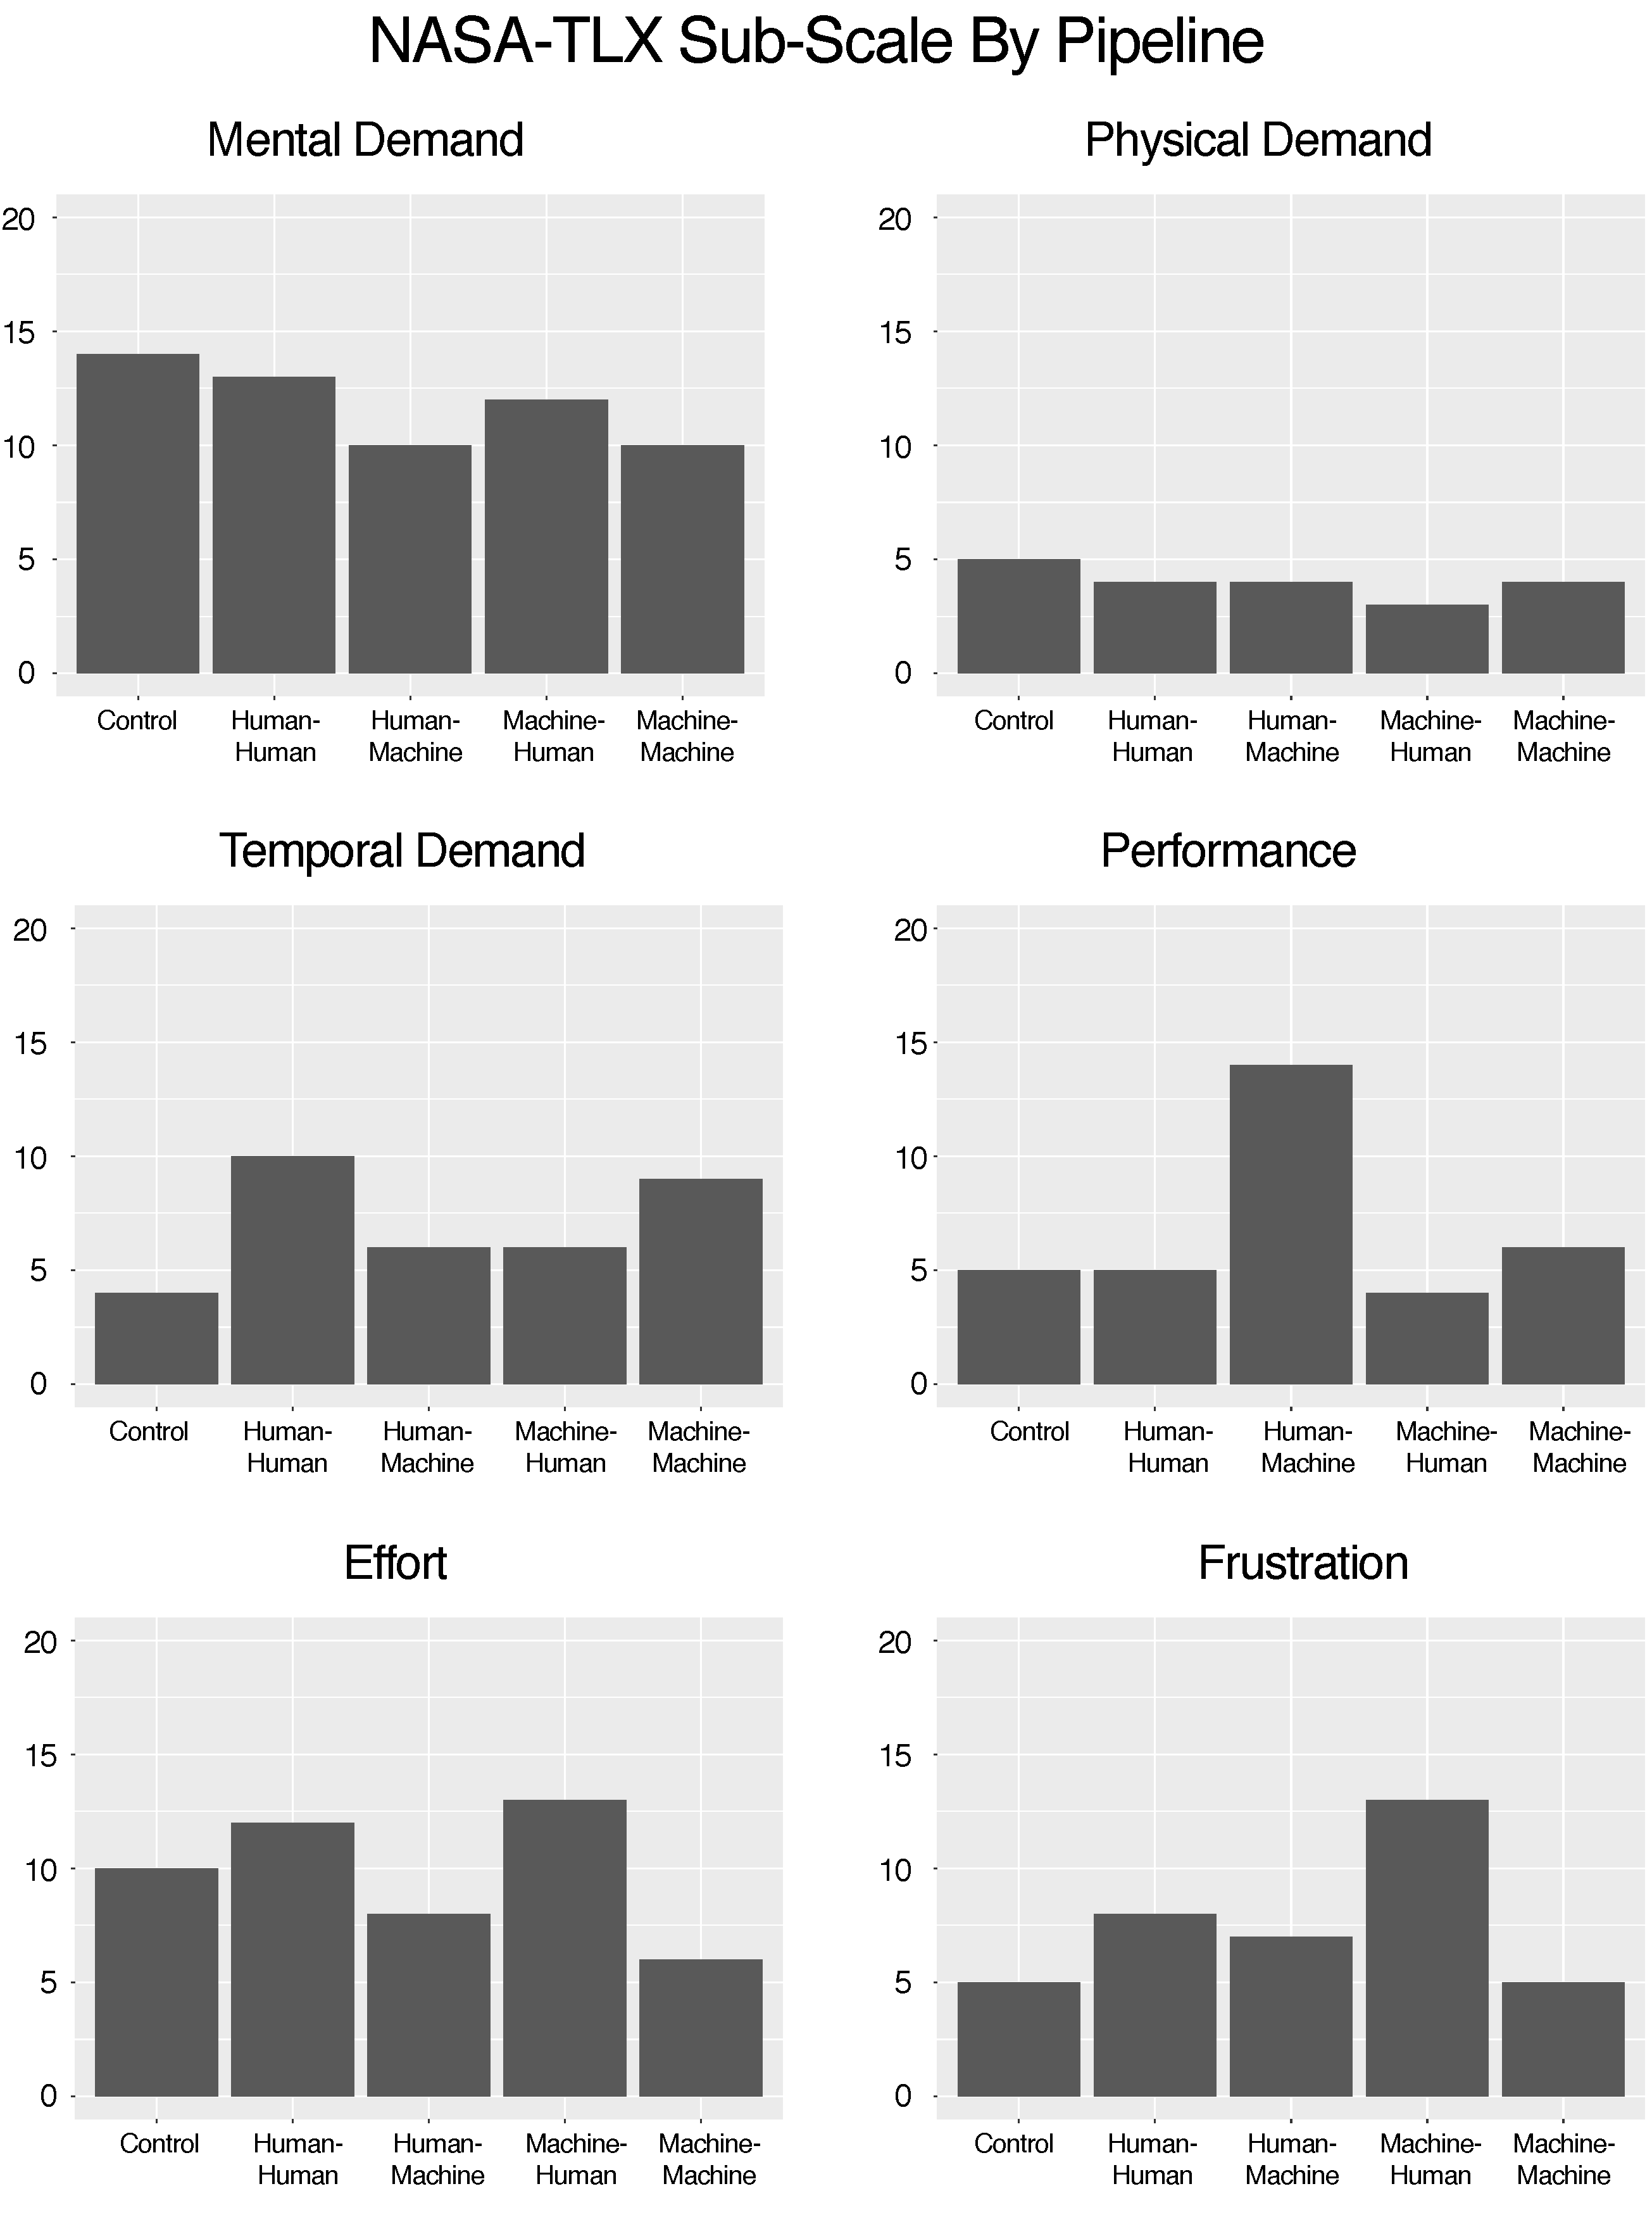
\includegraphics[width=\textwidth]{images/plot_tlx.pdf}
  \caption{NASA-TLX scores by sub-scale}
  \label{fig:plot:tlx}
\end{figure}

\begin{table}[htbp]
  \centering
  \caption{Kruskal-Wallis analysis of variance by pipeline for NASA-TLX survey}
  \label{tab:tlx}
  {\tabulinesep=2mm
    \begin{singlespace}
    \begin{tabu} to 0.6\textwidth{|X[c]|X[c]|X[c]|}
        \hline
        Sub-Scale & $\chi^2$ & $p$ \\
        \hline\hline
        Mental Demand & $\chi^2(4) = 2.53$ & $0.64$ \\
        \hline
        Physical Demand & $\chi^2(4) = 0.25$ & $0.99$ \\
        \hline
        Temporal Demand & $\chi^2(4) = 1.01$ & $0.91$ \\
        \hline
        Perceived Performance & $\chi^2(4) = 1.99$ & $0.74$ \\
        \hline
        Effort & $\chi^2(4) = 0.92$ & $0.92$ \\
        \hline
        Frustration & $\chi^2(4) = 3.59$ & $0.46$ \\
    \hline
    \end{tabu}
    \end{singlespace}
    }
\end{table}

We found no evidence to suggest that pipeline affects any of the NASA-TLX sub-scales.

In addition to the NASA-TLX survey, after each route leg we administered a three-question Likert scale survey addressing the quality of landmarks selected by the pipeline and the confidence subjects felt at navigational decision points. Each question is a statement with which the subject indicates their agreement, selecting from \textit{strongly agree}, \textit{agree}, \textit{not sure}, \textit{disagree}, and  \textit{strongly disagree}. The statements are as follows:

\textit{The landmarks I was told about helped me find turns.}

\textit{I knew what each landmark was going to look like when I heard its description.}

\textit{I felt confident in where to perform each maneuver (turn) on the route.}

In Figure \ref{fig:plot:likert} we show the distribution of agreement with each statement by pipeline. Each color represents a different score, with the lightest equating to \texit{``strongly disagree"} and the darkest to \texit{``strongly agree"}. The more width a color occupies, the more subjects gave that answer as their response.

In Table \ref{tab:likert} we analyze these results using a Kruskal-Wallis test to determine if there are significant differences in the distribution of answers between pipelines. For each survey question, we rejected the null hypothesis at significance level of 0.10; there is evidence that pipeline does affect participant responses to each of these questions. 

\begin{figure}[htbp]
  \centering
  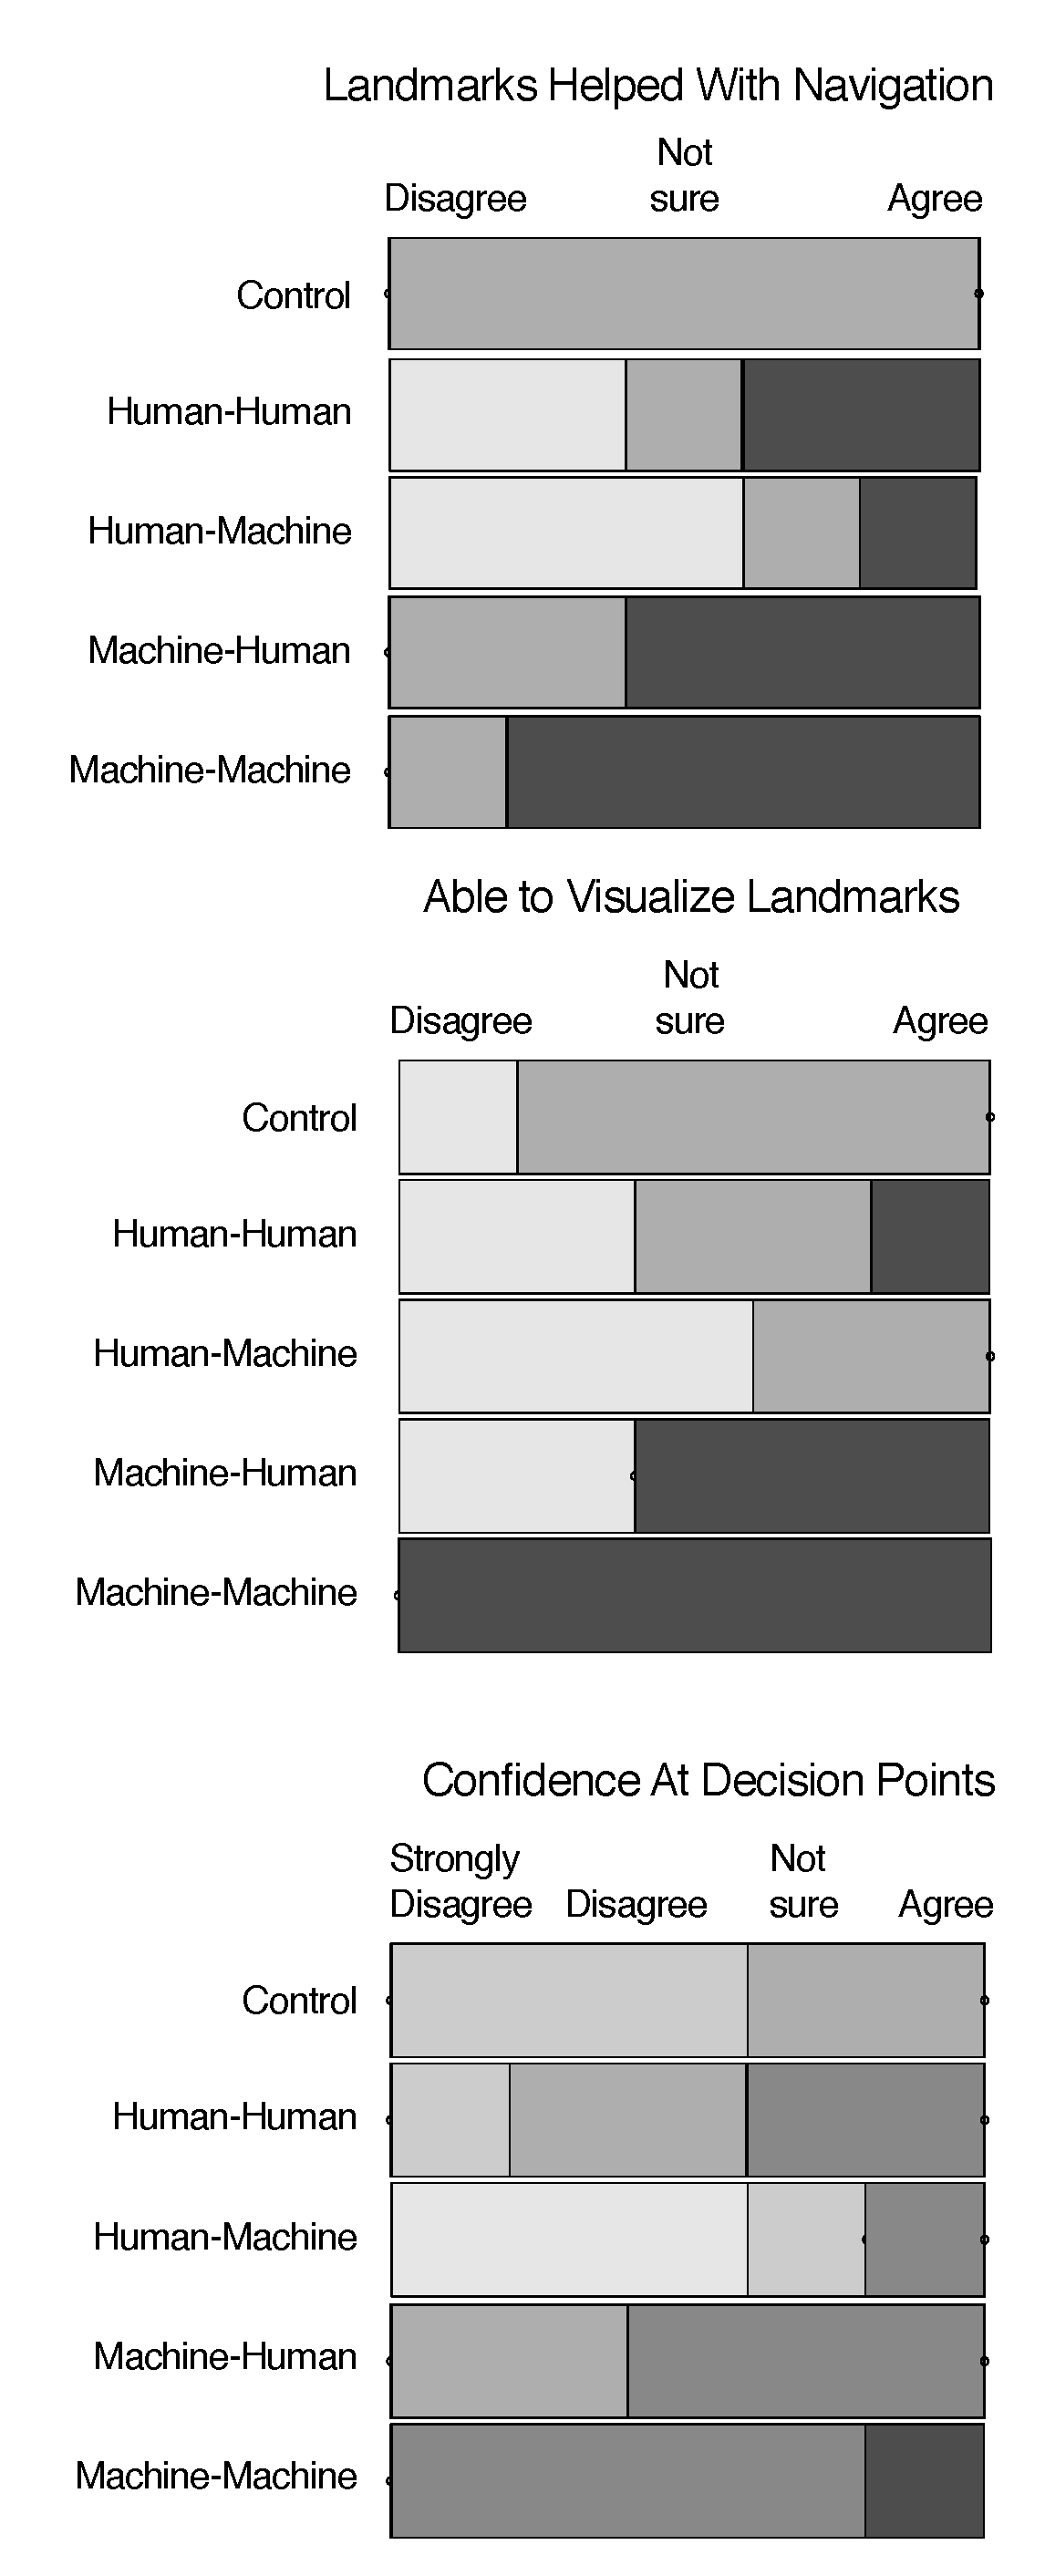
\includegraphics[width=0.5\textwidth]{images/plot_likert.pdf}
  \caption{Landmark effectiveness survey scores}
  \label{fig:plot:likert}
\end{figure}

\begin{table}[htbp]
  \centering
  \caption{Kruskal-Wallis analysis of variance by pipeline for landmark survey}
  \label{tab:likert}
  {\tabulinesep=2mm
    \begin{singlespace}
    \begin{tabu} to \textwidth{|X[c]|X[c]|X[c]|}
        \hline
         Question & $\chi^2$ & $p$ (* denotes significance at the 0.1 level) \\
        \hline\hline
        Landmarks helped find turns & $\chi^2(4) = 8.11$ & $0.08^*$ \\
        \hline
        Landmarks could be visualized from descriptions & $\chi^2(4) = 10.64$ & $0.03^*$ \\
        \hline
        Subject was confident at decision points & $\chi^2(4) = 13.83$ & $0.01^*$ \\
    \hline
    \end{tabu}
    \end{singlespace}
    }
\end{table}

In order to determine which pipelines are significantly different from others in terms of their affect on each survey question, we use Dunn's test with a Bonferroni adjustment for post-hoc analysis. Dunn's is a pairwise comparison test which, for each combination of pipelines $(a, b)$, tests the null hypothesis that the probability of drawing a larger value from $a$ than from $b$ is 0.5. The alternative hypothesis is that one group stochastically dominates another: the chances of sampling a larger value form that group is greater than 0.5. The Bonferroni adjustment adjusts $p$-values to account for having done multiple comparisons.

For the ``confidence at decision points" metric, we find that Machine-Machine pipeline is significantly more likely to have a higher (more agreeable) score than the control pipeline ($Z=-2.78$, $p=0.05$) as well as the Human-Machine pipeline ($Z=-3.21$, $p=0.01$). For the ``landmarks helped find turns" metric, we find no evidence of significant differences in distribution between two specific pipelines. For the ``landmark descriptions" metric we we find that Machine-Machine pipeline is significantly more likely to have a higher (more agreeable) score than the human-machine pipeline ($Z=-3.02$, $p=0.02$).

\subsection{Discussion}
Contrary to existing literature, we did not find the inclusion of landmark descriptions in navigation instructions to have a significant effect on drivers' cognitive load, erratic driving behavior, or perceived task load. We did find that instructions inclusive of landmark descriptions generated entirely by machine (machine-machine pipeline) lead to increased driver confidence at decision points as compared to navigation instructions which included only street name and distances (control pipeline). This finding is in line with participants' subjective written comments, which indicated that including stop lights and stop signs in instructions was helpful.

Without a larger study, it is not possible to definitely say whether or not any of Torchbearer's pipelines were effective in terms of reducing cognitive load, harsh G-force events or perceived task load. While we found no evidence of such effects in our small field study, a larger study, preferably consisting of 30 participants, would offer more definitive insight.

\section{Threats to Validity}

As alluded to previously, the principal threat to validity is the extremely small sample size employed in our field experiments. However, even within this small-scale study there are potential biases: first, study participants had relatively high familiarity with area of the route, given that all were residents of Bozeman, Montana. If landmark descriptions are more helpful in terms of cognitive load, erratic driving reduction or reduced task load in areas drivers are unfamiliar with, we would significantly underestimate the effect.

Due to time constraints, and the instrumented-vehicle experiment as opposed to a simulated one, each leg of the test route did not include a large number of maneuver points. Additionally, there was little variation in terms of road and environment type (surface versus highway, urban versus rural). A simulator-based experiment could allow for efficiently varying the driving environment.

Subjects may have been predisposed to "like" the concept of including landmarks in navigation instructions, even if there was no observable effect in terms of workload or driving behavior. This could potentially bias the results of the "confidence at maneuver points" survey---if subjects felt like they were "supposed" to like landmarks, they may have been inclined to indicate an increased sense of confidence.